
\documentclass[12pt,a4paper]{report}
\usepackage[export]{adjustbox}
\usepackage{booktabs}
\usepackage{amsmath}
\usepackage{amsfonts}
\usepackage{color,eurosym}
\usepackage{amssymb}
\usepackage{float}
\usepackage{graphicx}
\usepackage[hyphens]{url}
\usepackage{hyperref}
\usepackage{enumitem}
\usepackage[table,xcdraw]{xcolor}
\hypersetup{
    colorlinks,
    citecolor=blue,
    filecolor=blue,
    linkcolor=blue,
    urlcolor=blue
}
\newtheorem{remark}{\textbf{Remark}}[section]
%Cambiar los colores de blue a black para la impresion final

%\topmargin -1cm
%\textheight 24cm
%\oddsidemargin -0.5cm
%\textwidth 17cm

\begin{document}

%PRIMERA PAGINA: La portada
\thispagestyle{empty}

\begin{figure}[h]
  	\centering
  	 
\includegraphics[width=0.3\textwidth]{IMG/escudo_upv_transp.pdf}
\end{figure}
\begin{center}
\textbf{\normalsize Universitat Polit\`{e}cnica de Val\`{e}ncia}\\
\textbf{\normalsize Departament de Matem\`{a}tica Aplicada}

\vspace{1cm}

\scriptsize{\textbf{PhD. THESIS}}

\vspace{0.5cm}

\begin{center}
\textbf{\Huge Building networks of sexual partners. Application for the study of the transmission dynamics of Human Papillomavirus (HPV)}
\end{center}

\vspace{3cm}

\begin{tabular}{ccc}
\textbf{Ph.D. CANDIDATE} 				& \hspace{0.7cm} &\textbf{ADVISORS} \\
 										& \hspace{0.7cm} &\\
 										& \hspace{0.7cm} &\normalsize{Dr. Luis Acedo Rodr\'{i}guez \hfill} \\
										& \hspace{0.7cm} &\\
\normalsize{V\'{i}ctor S\'{a}nchez Alonso} 	& \hspace{0.7cm} & \normalsize{Dr. Rafael Jacinto Villanueva Mic\'{o} \hfill } \\ 
										& \hspace{0.7cm} &\\
 										& \hspace{0.7cm} & \normalsize{Dr. Francisco Javier Villanueva Oller \hfill} \\ 
\end{tabular} 

\vspace{2cm}

\normalsize{\textbf{Valencia - October 2017}}

\end{center}

\newpage

%SEGUNDA PAGINA: El certificado

\vspace{3cm}
Dr. Luis Acedo Rodr\'{i}guez and Dr. Rafael Jacinto Villanueva Mic\'{o}, from the Universitat Polit\`{e}c\-ni\-ca de Val\`{e}ncia and Dr. Francisco Javier Villanueva Oller from the Universidad Rey Juan Carlos,
\vspace{1.5cm}

\textbf{CERTIFY} that the present thesis entitled \textit{Building networks of sexual partners. Application for the study of the transmission dynamics of Human Papillomavirus (HPV)} has been performed under our supervision in the Department of Applied Mathematics at the Universitat Polit\`{e}cnica de Val\`{e}ncia by V\'{i}ctor S\'{a}nchez Alonso. It constitutes his thesis dissertation to obtain the PhD degree in Mathematics.

In compliance with the current legislation, we authorize the presentation of this dissertation signing the present certificate.

\vspace{1.5cm}

\begin{center}
Valencia, \today
\end{center}

\vspace{5cm}

\begin{center}
\begin{tabular}{ccccc}
Luis & \hspace{1.4cm} & Rafael Jacinto	& \hspace{1.4cm} &  Francisco Javier  \\
Acedo Rodr\'{i}guez & \hspace{1.4cm} & Villanueva Mic\'{o}	& \hspace{1.4cm} &  Villanueva Oller 
\end{tabular} 
\end{center}

\newpage

%TERCERA PAGINA: Los resumenes

\chapter*{Abstract}
Sexually Transmitted Diseases (STD) have been a major public health threat for a long time in human history. Modern concerns about STD began with the pandemic of syphilis which spread over Europe in the early sixteenth century. 

The Human Papillomavirus (HPV) is the direct cause of more than half million new cases of cervical cancer, the second most common malignancy among women and a leading cause of cancer death worldwide. It also causes anogenital warts. It is estimated that the probability of transmission of HPV is 40-50\% per contact. The networks of sexual contacts in human populations are crucial to the spread of sexually transmitted diseases (STDs).

Working in large networks applied to epidemiological-type models has led us to design a simple but effective computed distributed environment to perform a large amount of model simulations in a reasonable time in order to study the behavior of these models and to calibrate them. Finding the model parameters that best fit the available data in the designed distributed computing environment becomes a challenge and it is necessary to implement reliable algorithms for model calibration.

We are able to simulate our model and carry out vaccination campaigns in order to get conclusions concerning the best strategies. This information can be useful for Health Care, policy makers and pharmacological industries to save time and money.


\chapter*{Resum en Valenci\`a}

\newpage

%INDICES
\tableofcontents
\listoffigures
\listoftables

%El cap�tulo 1 debe ser la introducci�n al VPH que ya redactaste. 
%El cap�tulo 2 debe describir la construcci�n de la red y la din�mica de transmisi�n como est� en el art�culo de viruses. 
%El cap�tulo 3 debe ser el 2 del git de arriba donde se describe el calibrado. 
%El cap�tulo 4 el 3 del report donde se describe la red din�mica y la vacunaci�n. 
%El cap�tulo 5 de la tesis deber�a ser el caso australiano tal cual del art�culo de viruses.

%Cap�tulo 1 - ya redactado

\chapter{Introduction}\label{intro}

\section{The revelation of the virus}
%Algo importante que contar
One of the biggest scientific discoveries in the past 30 years was the connection between human papillomavirus infection of the cervix and cervical cancer. This achievement resulted from the original seminal findings by Harald zur Hausen and his group, they found that human papillomavirus genotype 16 can be detected in cervical cancer tissue. 
\begin{figure}[ht]
	\centering
	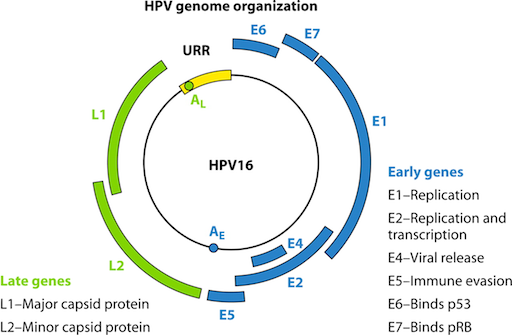
\includegraphics[scale=0.7]{IMG/genoma.png}
	\caption{Cartoon illustrating the genomic organization of a typical mucosal high-risk HPV. The genome contains early and late regions (E), which relate to the positions of the genes within the genome and their timing of expression during the viral life cycle. The early region carries a number of genes which function at the level of viral replication and transcription, i.e., E2, E1, E6, and E7. E2 encodes a protein which has an auxiliary role in viral replication and also functions at the level of transcriptional regulation of the viral early genes. The E6 and E7 genes encode the major transforming proteins of the oncogenic HPVs. The late region (L) encodes viral structural proteins, with L1 being the major capsid protein and L2 being the minor capsid protein.}
	\label{genoma}
\end{figure}
%doi: 10.1128/CMR.05028-11 Clin. Microbiol. Rev. April 2012 vol. 25 no. 2 215-222 1 April 2012

%Foto del HPV-16 con Cryo-EM (nobel química 2017)

The finding was followed by epidemiologists, molecular biologists, vaccinologists, and clinicians culminating in 2006 with the development of effective prophylactic vaccines for human papillomavirus, which have the means to prevent 70-80\% of cervical cancer. Zur Hausen was awarded the Nobel Prize in Physiology or Medicine in 2008, in recognition of his discovery.

\begin{figure}[ht]
	\centering
	
\includegraphics[scale=0.7]{IMG/zurHausen.png}
	\caption{Harald zur Hausen (born 11 March 1936) is a German virologist and professor emeritus. He has done research on cancer of the cervix, where he discovered the role of papilloma viruses, for which he received the Nobel Prize in Physiology or Medicine 2008.}
	\label{zurHausen}
\end{figure} 
%Foto de Zur Hausen

%Datos de lo malo que es
HPV types are often referred to as low risk (LR) wart causing or high risk (HR) cancer causing, based on whether they put a person at risk for cancer.  The types of HPV that can cause genital warts are not the same as the types that can cause cancer.
Persistent human papillomavirus (HPV) infections with genotypes 16 and 18 are responsible for about 70\% of all cervical cancer 
%Clifford GM, Rana RK, Franceschi S, Smith JS, Gough G, Pimenta JM. Human papillomavirus genotype distribution in low-grade cervical lesions: comparison by geographic region and with cervical cancer. Cancer Epidemiol Biomarkers Prev. 2005;14:1157–1164. doi: 10.1158/1055-9965.EPI-04-0812.
%Munoz N, Bosch FX, de Sanjosé S, Herrero R, Castellsague X, Shah KV, et al. Epidemiologic classification of human papillomavirus types associated with cervical cancer. N Engl J Med. 2003;348:518–527. doi: 10.1056/NEJMoa021641.
, with 40-85\% of other anogenital cancers: anal, penile, vaginal, and vulvar cancer, and also 16-28\% of the head and neck cancers.
%%WHO International Agency for Research on Cancer. IARC Monographs on the Evaluation of Carcinogenic Risk to Humans. Human Papillomavirusses. Volume 90. 2007.
%https://www.ncbi.nlm.nih.gov/pmc/articles/PMC4331443/

HPV is a cause of other non malignant diseases, to mention genotypes 6 and 11 cause about 90\% of anogenital warts, and secondarily juvenile onset of recurrent respiratory papillomatosis.
%Lacey CJ, Lowndes CM, Shah KV. Chapter 4: Burden and management of non-cancerous HPV-related conditions: HPV-6/11 disease. Vaccine. 2006;24(Suppl 3):S35–S41. doi: 10.1016/j.vaccine.2006.06.015.

% Literatura dura
Genital human papillomavirus (HPV) is the most common sexually transmitted infection in the United States. More than 40 HPV types can infect the genital areas of men and women, including the skin of the penis, vulva (area outside the vagina), and anus, and the linings of the vagina, cervix, and rectum. These types can also infect the lining of the mouth and throat.

\begin{figure}[ht]
	\centering
	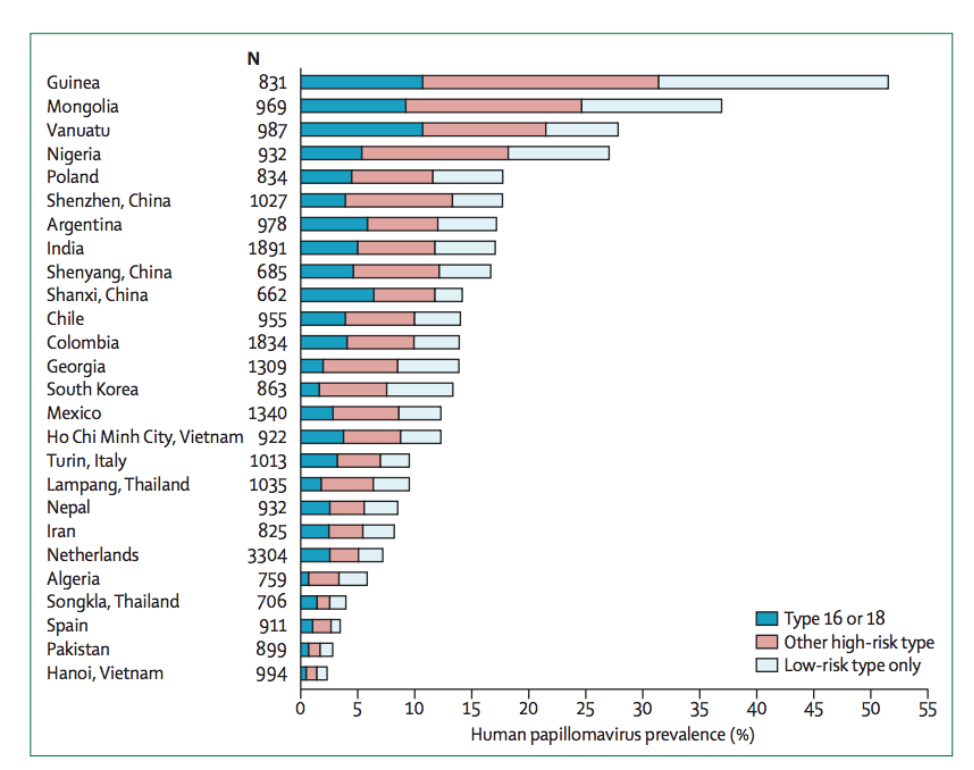
\includegraphics[scale=0.7]{IMG/prevalence.png}
	\caption{Age\-adjusted prevalence of cervical human papillomavirus DNA in sexually active women aged 15\-69 years. Data are from IARC Prevalence Surveys, 1990\-2012.4}
	\label{zurHausen}
\end{figure} 
%Foto de prevalencia


%Literatura
Most people who become infected with HPV do not know they have it. Usually, the body's immune system gets rid of the HPV infection naturally within two years. This is true of both HR and LR types. By age 50, at least 4 out of every 5 women will have been infected with HPV at one point in their lives. HPV is also very common in men, and often has no symptoms.

When the body's immune system can't get rid of a HR HPV infection, it can linger over time and turn normal cells into abnormal cells and then cancer. About 10\% of women with HR HPV on their cervix will develop long-lasting HPV infections that put them at risk for cervical cancer. Similarly, when HR HPV lingers and infects the cells of the vulva, vagina, penis, anus, or the oropharynx (back of the throat, including the base of the tongue and tonsils), it can cause cell changes called precancers. These may eventually develop into cancer if they're not found and removed in time. These cancers are much less common than cervical cancer. Much less is known about how many people with HPV will develop cancer in these areas.

%Empiezo con las vacunas
\section{Vaccines}
Since the release of the first vaccines in 2006, nowadays there are three available: a quadrivalent (including HPV genotypes 16, 18, 6 and 11) and a bivalent vaccine (including genotypes 16 and 18) and a nonavalent (including genotypes 6, 11, 16, 18, 31, 33, 45, 52 and 58). All vaccines are efficacious to protect against precancerous lesions in the cervix, vulva or vagina; in addition, the quadrivalent and nonavalent prevent precancerous anal lesions, anal cancer and anogenital warts.

\begin{figure}[ht]
	\centering
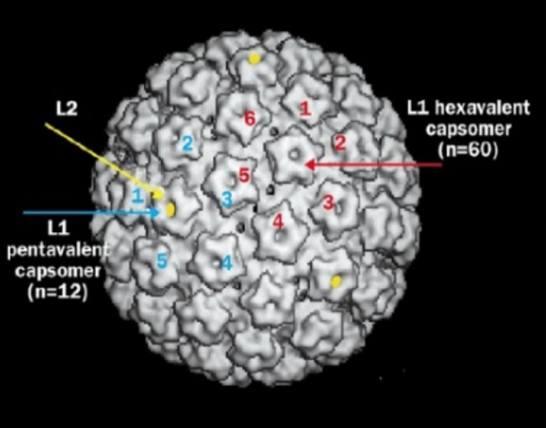
\includegraphics[scale=0.7]{IMG/cryo.png}
\caption{Structure of a HPV virus-like particle. A three-dimensional reconstruction of a cryolectron micrograph (cryo-EM) of a virus-like particle (VLP) is shown. The VLP is composed of 60 hexavalent capsomers and 12 pentavalent capsomers, all consisting of pentamers of L1 protein. The L2 protein is not visible by cryo-EM but is tought to be associated with the pentavalent capsomers, and have been colored in yellow.}
\label{cryo}
\end{figure}  

According to the Advisory Committee on Immunization Practices (ACIP) from the Centers for Disease Control (CDC) and Prevention, new recommendations are given for use of a 2-dose schedule for girls and boys who initiate the vaccination series at ages 9 through 14 years. Three doses remain recommended for persons who initiate the vaccination series at ages 15 through 26 years and for immunocompromised persons.

In Spain HPV vaccine is given to adolescent girls as part of the national immunization programme, and is recommended at different age groups in different Autonomous Communities. Numerous cost-effectiveness studies of HPV-vaccination have been published in other countries. However, few studies include the prophylactic effect of all HPV-associated diseases, or the impact of vaccinating men.

There are countries that recommend also vaccinating boys in order to decrease the burden of disease in them. Some models have shown that the female vaccination program has some herd immunity and the impact of implementing the vaccination in males may not be cost effective, however not vaccinating males leaves them at risk of cancers, especially the groups that do not benefit of the herd immunity, as the males that have sex with males.
Besides, there is no economic analysis of the nonavalent program in Spain, and it is important from the decision making perspective.

Even with the high prevalence of sexually transmitted diseases there are few studies devoted to ascertain the structure of sexual networks and its role in disease transmission. Most studies are restricted to small communities such as the Jefferson High Schools project (P. S. Bearman et al., Chains of Affection: The Structure of Adolescent Romantic and Sexual Networks, American Journal of Sociology, 110(1) (2004) 44-91) or that of Likoma Island (S. Helleringer and H. P. Kohler, Sexual network structure and the spread of HIV in Africa: evidence from Likoma Island, Malawi, AIDS 21 (2007) 2323-2332).

Random network mathematical models may simulate the interactions and propagations of all these viruses through sexual contacts among a population of more than one million people (including heterosexual and homosexual populations). As this model is based upon a network instead of traditional continuous model approaches (E. H. Elbasha et al., Model for assessing human papillomavirus vaccination strategies,  Emerging. Inf. Dis.  2007; 13:28-41) we will be able to determine with higher accuracy the effect of vaccination in a short and large periods of time.

The Human papillomaviruses HPV vaccine induces a herd immunity effect in genital warts when a large number of the population is vaccinated. This aspect should be taken into account when devising new vaccine strategies, like vaccination at older ages or male vaccination. Therefore, it is important to develop mathematical models with good predictive capacities. We devised a sexual contact network that was calibrated to simulate the Spanish epidemiology of different HPV genotypes. Through this model, we simulated the scenario that occurred in Australia in 2007, where 12-13 year-old girls were vaccinated with a three-dose schedule of a vaccine containing genotypes 6 and 11, which protect against genital warts, and also a catch-up program in women up to 26 years of age. Vaccine coverage were $73\%$ in girls with three doses and with coverage rates decreasing with age until $52\%$ for 20-26 year-olds. A fast $59\%$ reduction in the genital warts diagnoses occurred in the model in the first years after the start of the program, similar to what was described in the literature.


%Cap�tulo 2 - de revista Viruses
\chapter{Building LSP networks and describing the transmission dynamics of HPV on these networks}\label{ConstruccionYDinamica}

\section{Origin of the data}

%me enrollo un poco mas
Building a social network requires demographic data, for this model we have used data from the region of Valencia (Spain) that was collected from the Valencian Institute of Statistics (2013) \cite{IVE}, from this set of data we are interested in the distribution of males and females along with their age. The second set of data for this model has to do with sexual habits, this is the LSP for an individual, which was obtained from the Health and Sexual Habits Survey of 2003 \cite{INE}, and summarized in Table \ref{tableLSPValues}. 

\begin{table}[H]
\centering
\begin{tabular}{ccccccc}
\toprule
\multicolumn{7}{c}{\textbf{MALES}} \\ \midrule
\textbf{ Age} & \textbf{0 LSP} & \textbf{1 LSP} &\textbf{ 2 LSP} & \textbf{3--4 LSP} & \textbf{5--9 LSP} & \textbf{10 or More LSP} \\
\midrule
14--29 & 0.107 & 0.207 & 0.131 & 0.225 & 0.168 & 0.162 \\
30--39 & 0.027 & 0.225 & 0.128 & 0.21 & 0.17 & 0.24 \\
40--65 & 0.019 & 0.268 & 0.14 & 0.193 & 0.163 & 0.217 \\
 \midrule 
 
\multicolumn{7}{c}{FEMALES} \\ \midrule
  Age & $0$ LSP & $1$ LSP & $2$ LSP & 3--4 LSP & 5--9 LSP & $10$ or more LSP \\
 \midrule
14--29 & 0.138 & 0.43 & 0.186 & 0.158 & 0.056 & 0.032 \\
30--39 & 0.029 & 0.501 & 0.168 & 0.177 & 0.077 & 0.048 \\
40--65 & 0.017 & 0.652 & 0.138 & 0.118 & 0.039 & 0.036 \\
\bottomrule
\end{tabular} 
\caption{Proportion of males and females per number of life sexual partners {LSP} per age group. Note that the sum of the rows are 1}
\label{tableLSPValues} 
\end{table}

Some features of the distribution of contacts were: (i) the percentage of males and females with no partners is
very similar in each age-group; (ii) the proportion of women  with a single partner is, approximately, two times larger than men with only one partner; and (iii) the percentage of men with two or more partners is always larger than that of women except for women in the age-groups 14--29, and~30--39 in the case of two partners. The asymmetry in the behaviour of males and females should be taken into account in the construction of the network.

\section{Network model}

In this dissertation, we use the random network model as a basis to simulate the network of sexual contacts among individuals, but, in this model, the average number of connections depend upon the age-group as deduced from Table \ref{tableLSPValues}. A basic property of the network we are going to discuss is that the total number of LSP for the male population (M) must coincide with the total number of LSP for the female population (F). This is so because (in a purely heterosexual network) every link starting on a male must end in a female and viceversa. In mathematical terms:

\begin{equation}
\label{nodeseq}
\displaystyle\sum_{i=1}^M\, LSP_i=\displaystyle\sum_{j=1}^F\, LSP_j\; .
\end{equation}

The estimation of sexual partners: there are some approaches to the number of LSP in males and females \cite{chandra2013sexual,mosher2005sexual} that are difficult to match. Generally speaking, males tend to overestimate the number of their sexual partners and females tend to underestimate it. Therefore, we considered the average LSP male value, $\left\langle k \right\rangle_m$, and calibrated the network so that results were consistent with data of Table \ref{tableLSPValues}, and estimated that the number of LSP in males in Spain was at least $4.5$. Networks with 100,000, 250,000, 500,000 and 750,000 have been necessary to perform the present study. It required a substantial computational power.

\section{Semi-Random Construction}
\label{subsec22}

From Table \ref{tableLSPValues} (proportion of male LSP aged 14--29), we have the following list:
$( 0.107, 0.314, 0.445, 0.67, 0.838, 1)$ for the accumulated proportion of males less than or equal to a given LSP number.
Now, we randomly generate a number $r$ between $0$ and $1$ and assign the number of contacts to every male node in the $14-29$
age group, in the network as follows:

\begin{itemize}[leftmargin=*,labelsep=5mm]
\item $r \le 0.107$ say that the corresponding male does not have an LSP,
\item $0.107 < r \le 0.314$ say that the corresponding male has one LSP,
\item $0.314 < r \le 0.445$ say that the corresponding male has two LSPs,
\item $0.445 < r \le 0.67$  say that the corresponding male has three or four LSPs uniformly distributed.
\item $0.67 < r \le < 0.838$ say that the corresponding male has five to nine LSPs uniformly distributed.
\item $0.838 < r \le 1$ say that the corresponding male has 10 or more LSPs.
\end{itemize}

Every node in the network is labelled by its gender and age randomly assigned according to the population histogram. The assignment of the number of bonds, as another label of the node, is not so straightforward since we must guarantee that the condition in Equation\ (\ref{nodeseq}) is verified. In~order to fulfill this condition, we take advantage of the uncertainty of statistics reports concerning individuals with $10$ or more LSPs.

Starting with the males, we assign the number of LSPs up to nine partners and, for $10$ or more partners proceed as follows: let $i_{\mbox{max}}$ be the number of males with nine or less partners. The unassigned males should be $M-i_{\mbox{max}}$ and the number of bonds that should be distributed among them is $M \left\langle k \right\rangle_m-\sum_{i=1}^{i_{\mbox{max}}}\, LSP_i$. By Euclidian division, this quantity can be expressed as $(M-i_{\mbox{max}}) n_m+r_m$, where $n_m \ge 10$. In our procedure, we assign a random number of bonds, uniformly distributed, in the interval $\left[10,2 n_m-10\right]$ to every male with $10$ or more LSPs, i.e.,
to~the $M-i_{\mbox{max}}$ unassigned males.

Now, we denote as $p_m$ the total number of bonds of the male population. We must take into account, as expressed in Equation\
(\ref{nodeseq}), that the total number of bonds of the female population should be the same. To impose that condition, we
proceed as follows: (i) assign the number of bonds to the females with nine or less partners following the statistical 
data in Table \ref{tableLSPValues}; and (ii) the sum of all female LSPs in this group of $j_{\mbox{max}}$ members will be denoted by $s_f$. 
Then, $n_f=F-j_{\mbox{max}}$ is the number of females with $10$ or more LSPs; and (iii) the number of bonds starting in the males and still unassigned to a female is $p_m-s_f= q_f n_f + r_f$, where $0 \le r_f < n_f$ and $n_f \ge 10$. (iv) We assign $q_f+1$ bonds to $r_f$ females still unassigned and $q_f$ bonds to the rest of $n_f-r_f$ females. The steps of this algorithm are also enumerated in the flow diagram in Figure  \ref{flux1}.

Notice that, for men and women with more than 10 LSPs, we assign their LSP in the most equitable way, assuming that all of them have, more or less, the same number of LSPs. Thus, we have a lot of hubs with a low number of contacts instead of a few hubs with a lot of contacts.

From the point of view of STD transmission, the latter situation leads to a faster transmission if the hub is infected, and, also, if the hub is vaccinated, the transmission is cut faster. Therefore, due to the lack of data about people with $10$ or more LSPs, we make the decision of being conservative in the transmission of the disease and in the effect of the vaccination campaigns.

Notice that this procedure implies that the condition in Equation\ (\ref{nodeseq}) is verified. After this procedure, we have obtained the following lists:
\begin{itemize}[leftmargin=*,labelsep=5mm]
\item $AgeMale\left[ i \right]$ is the age of the i-th male, $i=1,\ldots,M$,
\item $AgeFemale\left[ i\right]$ is the age of the i-th female, $i=1,\ldots,F$,
\item $kMale\left[ i \right]$ is the number of LSP for the i-th male, $i=1,\ldots,M$,
\item $kFemale\left[ i \right]$ is the number of LSP for the i-th female, $i=1,\ldots,F$.
\end{itemize}

\begin{figure}[H]
\centering
\begin{tabular}{c}
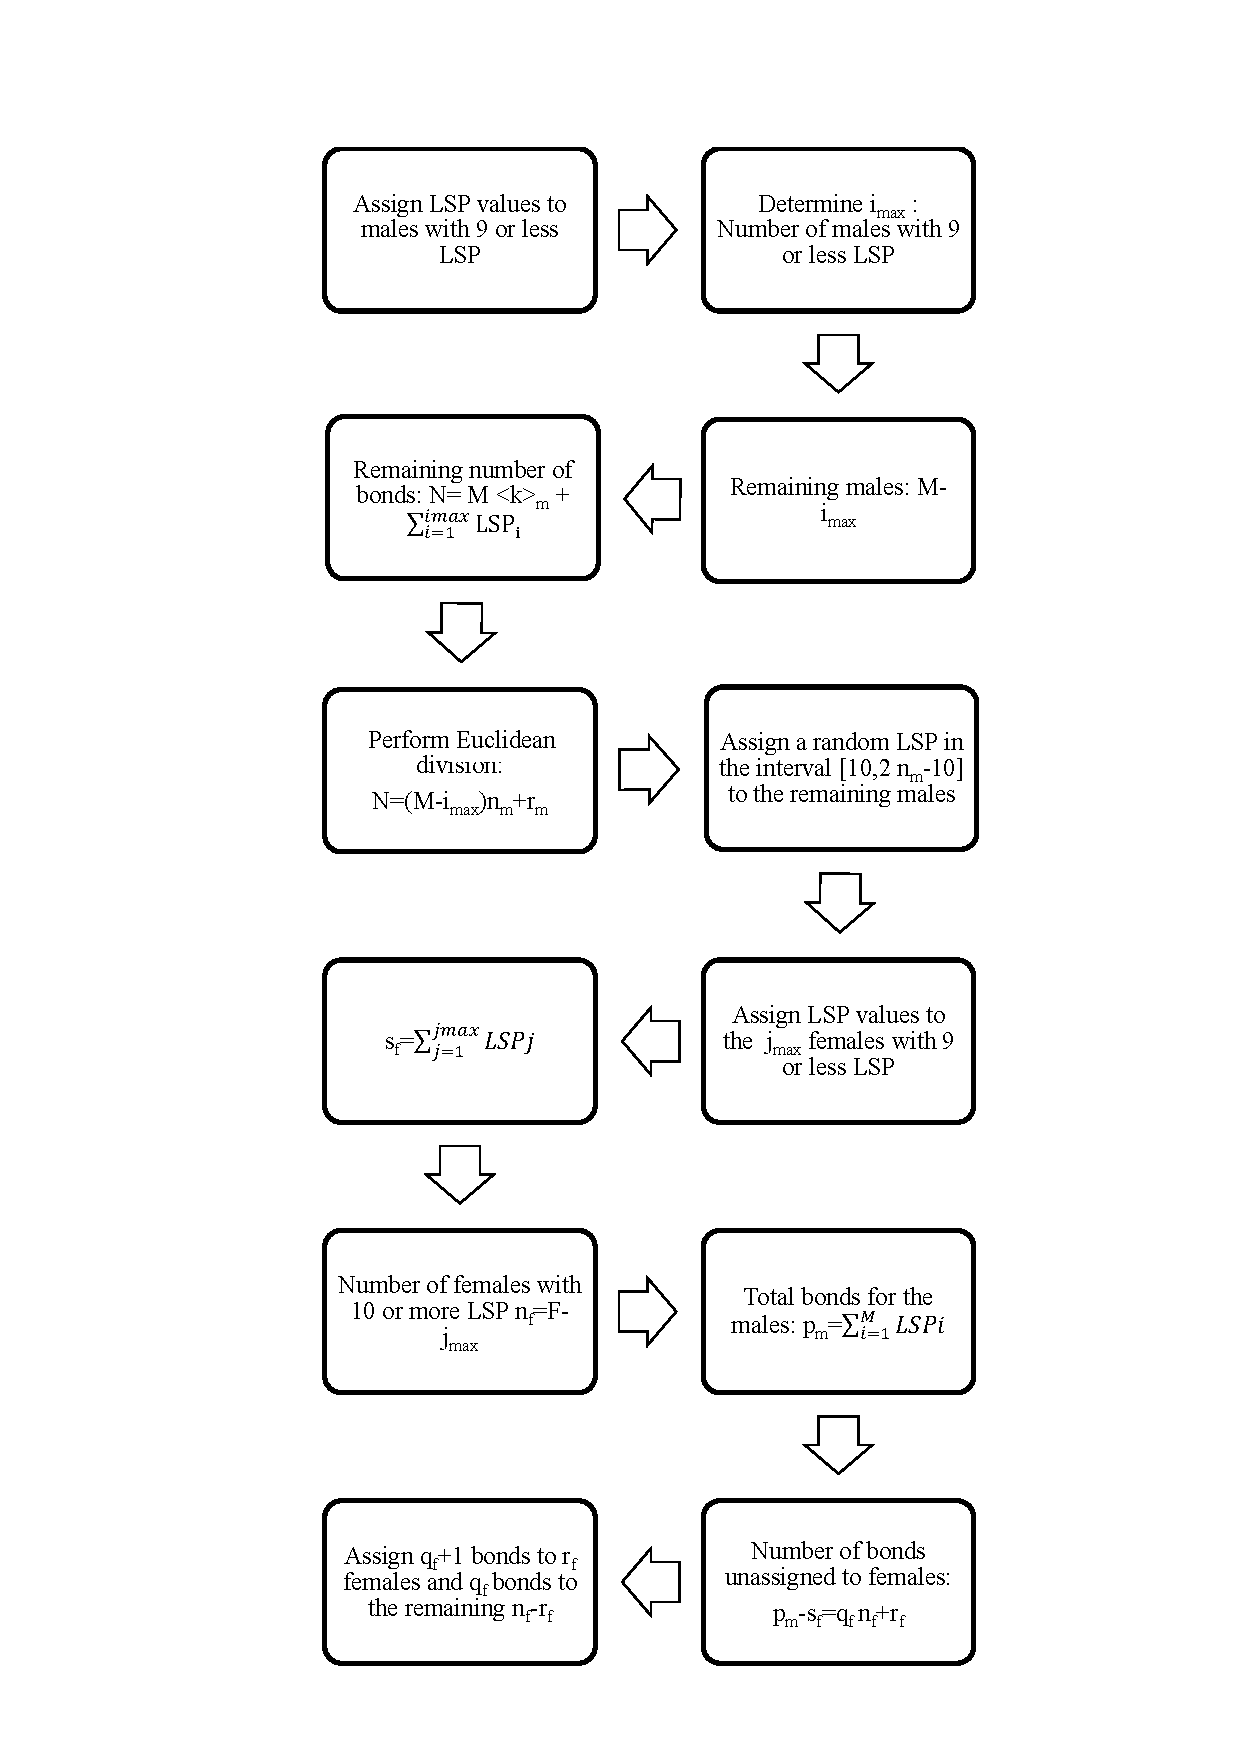
\includegraphics[width=\textwidth]{IMG/FluxDiagramI.pdf}
\end{tabular}
\caption{Flow diagram for the algorithm corresponding to the assignment of a number of LSPs to every male and female in the network.\label{flux1}}
\end{figure}

These lists will be used to perform the connections of males and females and build the network.
Note that, in Table \ref{tableLSPValues}, there are more females than males with few LSPs (comparing male and female percentages). It implies that there will be few women with a very large number of LSPs. This fact suggests us to start the assignment procedure with women with the largest LSPs. Otherwise, it would be possible that, when we have to assign LSPs of men to a female with a large number of LSPs, there~will not be enough men with free sexual partners to be assigned and, for this female, it would be impossible to satisfy the condition that the degree of each node was the number of its LSP. 

The assignment of partners was carried out by considering a principle of psychological similarity~\cite{gentner1997structure} or assortativity.
Hence, we are going to define a weight function assuming that: women with few LSPs usually match men with few LSPs; people with four or more LSPs use to join with people with four or more LSPs; and couples where one of them has a large number of LSPs and the other few LSPs will be uncommon. Then, for the woman $i$ and the man $j$, we define the following weight~function:

\begin{equation}
\pi(i,j) = 
\begin{array}{l}
\left\lbrace \begin{array}{lc}
| kFemale[i] - kMale[j] | & kFemale[i], kMale[j] \le 4 \\
0 & kFemale[i], kMale[j] > 4 \\
100 & \mbox{otherwise}
\end{array} \right\rbrace, \\
\\
 + | AgeFemale[i] - AgeMale[j] - 1.8 |.
\end{array}
\label{peso}
\end{equation}

The combined weight function, which takes into account the age difference of the partners, $\vert AgeFemale[i] - AgeMale[j] - 1.8 \vert$ is defined in this way because some studies show that the average age difference among the members of a couple in Spain is $1.8$ years \cite{miret2010similitud}. 

%The MSM population (around $3.88$ \% of the total male population in Spain)\cite{INE} can also be incorporated into the model, but, in this subpopulation, the connectivity would be larger than the heterosexual network. The MSM population would also be connected with the heterosexual one by links with women in such a way that every MSM individual has a link with a woman with five or more contacts \cite{acedo2017calibrating}.

The estimated percentage of homosexual men is $3.88$ \%\cite{INE}. The situation for the homosexual men population is different of the one shown in Table \ref{tableLSPValues}, because the average number of sexual partners is estimated in 39 regardless of age, but this number increases with age with a peak of 59 in the 40-49 age-group \cite{Durex2002}.
A difficulty arises because we have little information about the number of sexual contacts in homosexual women subpopulation. In a personal communication by Dr. Mireia D\'iaz from the Catalan Institute of Oncology (IDIBELL) we were informed that HPV hardly spreads among homosexual women, and almost all homosexual men, sometimes in their lives, had a woman partner. Consequently, we have simulated these connections by assigning a contact to every man in the homosexual subpopulation with woman with 5 partners or more. This is done according to the assortativity principle, that is, people use to join with people with similar habits.

The assignment of links is then performed by the a Greedy Randomized Adaptive Search Procedure (GRASP) algorithm \cite{cormen2009introduction,feo1995greedy}. %Details about the construction of the whole network have been provided in previous studies \cite{acedo2017calibrating,BuildingLSPNova}. 


%Cap�tulo 3 - calibrado del articulo Report HPV RJVM August 25, 2018
\chapter{Calibrating the Sexual Contacts Network }\label{Calibrado}

\section{Calibration}
We already have performed a calibration published in \cite{Acedo2017}. This calibration allowed to reproduce the Australian scenario \cite{DezDomingo2017} where 12-13 years old girls were vaccinated and a catch-up vaccination on women aged 14-26 years old during two years was done. Two years after the vaccine was introduced, the proportion of genital warts diagnosed declined by a 59\% in vaccine eligible young women aged 12–26 years in 2007, and by 39\% in men of the same age.

However, the calibration of this kind of random computational models is an open problem and several issues about fitting computational models to data with uncertainty have to be addressed. For instance, 

\begin{itemize}
	\item the fact that, for the same set of parameters, different realizations usually return different outputs, and consequently, one realization may fulfill the fitting requirements and another realization does not,
	\item the determination of an appropriate measure of goodness-of-fit,
	\item to find model parameters agreeing the values appearing in the medical literature in a reliable and reproducible way,
	\item adaptation of the optimization algorithms to these above issues and the available resources,
	\item the determination of the best parallel implementation of the optimization algorithms, in terms of quality of the solutions and computational efficiency of the program.
\end{itemize} 

In the remainder of this section, we are going to describe thoroughly the procedure we propose to approach the above issues.

\subsection{Description of the model}\label{sec:modelo}
In the papers \cite{Acedo2017,DezDomingo2017}, we described how to build lifetime sexual partners (LSP) networks. These networks are built with the main aim to reproduce the demography in Spain, \cite{pegv} and data about the LSP, for men and women, and for age groups $18-29$, $30-39$ and $40-65$, presented in a survey about sexual habits in Spain \cite{INE} and collected in Table \ref{tableX}. 

\begin{table}[h]
	\centering
	\begin{tabular}{|c|c|c|c|c|c|c|}
		\multicolumn{7}{c}{MALES} \\
		\hline
		Age & $0$ LSP & $1$ LSP & $2$ LSP & $3-4$ LSP & $5-9$ LSP & LSP $\ge 10$ \\
		\hline
		$14-29$ & 0.107 & 0.207 & 0.131 & 0.225 & 0.168 & 0.162 \\
		$30-39$ & 0.027 & 0.225 & 0.128 & 0.21 & 0.17 & 0.24 \\
		$40-65$ & 0.019 & 0.268 & 0.14 & 0.193 & 0.163 & 0.217 \\
		\hline 
		\multicolumn{7}{c}{FEMALES} \\
		\hline
		Age & $0$ LSP & $1$ LSP & $2$ LSP & $3-4$ LSP & $5-9$ LSP & LSP $\ge 10$ \\
		\hline
		$14-29$ & 0.138 & 0.43 & 0.186 & 0.158 & 0.056 & 0.032 \\
		$30-39$ & 0.029 & 0.501 & 0.168 & 0.177 & 0.077 & 0.048 \\
		$40-65$ & 0.017 & 0.652 & 0.138 & 0.118 & 0.039 & 0.036 \\
		\hline
	\end{tabular} 
	\caption{Proportion of males and females per number of LSP per age group \cite{INE}. Note that the sum of the rows are 1.}
	\label{tableX} 
\end{table}

There are a lot of possible combinations to create networks fulfilling the above requirements. This fact makes that the built networks contain uncertainty in the sense of the randomness of the building process and the different shapes these networks may have. 

Then, over the LSP network, we describe the dynamics of the HPV \cite{Acedo2017,DezDomingo2017}. We divide the nodes into the age groups $14-17$, $18-29$, $30-39$, $40-65$. In order to describe properly the transmission dynamics of HPV on the LSP networks, it is necessary to include $11$ model parameters that will govern the aforementioned HPV dynamics:

\begin{enumerate}
	\item Average number of men LSP, 
	\item Global probabilities in order to determine if the existence of a LSP implies sexual intercourses in the current time step per age group $14-17$, $18-29$, $30-39$ and $40-65$ (4 parameters),
	\item Average time an individual infected by a high (low) risk HPV clears the infection and recovers (2 parameters)
	\item Probability that a woman (man) infected of high (low) risk HPV transmits it to his/her partner in a sexual intercourse (4 parameters). 
\end{enumerate}

Most of the above parameters have been studied in the literature and there are some estimations we have to take into account:
\begin{itemize}
	\item The average number of men LSP: it is around $8$ \cite{Durex2002}. For this parameter, our search will be in the interval $[7, 10]$.

	\item The time for clearing the infections due to HPV HR, for both men and women: in \cite{elbasha2007model}, the authors say that the mean duration of HPV 16/18 infection is $1.2$ years; in \cite{Giuliano2011}, the mean duration of HPV 16 is $12.19$  months $(7.16–18.17)$; in \cite{Nyitray2015} the duration clearance varies, in average, between $6.5$ months to $11.8$ months. Thus, we considered the interval $[0.8, 1.2]$ years.
	
	\item The time for clearing the infections due to HPV LR, for both men and women: in \cite{elbasha2007model}, the mean duration of HPV 6/11 infection is $0.7$ years; in \cite{Giuliano2011}, the mean duration of HPV infection is $7.52$ months $(6.80–8.61)$ for any HPV;  in \cite{Nyitray2015} the duration clearance varies, in average, between $6.2$ months to $11.7$ months. Thus, we considered the interval $[0.5, 1]$ years.
	
	\item In \cite{elbasha2007model}, the authors estimated the probability of HPV infection transmission per partnership and by type and, as in \cite{castellsague2012prevalence}, this probability is higher for transmission from males to females $(0.8)$ than that for transmission from females to males $(0.7)$. Given that these data come from estimations (not surveys) and after some runs of our model, we are going to be more flexible and consider the probability interval $[0.2,0.6]$ for LR transmission and $[0.5,1.0]$ for HR transmission, given that, women transmit less than men.
\end{itemize}

Now, we are able to define the dynamics of HPV. Setting the time step in a month, for every month:

\begin{itemize}
	\item  For each node $i$
	\begin{itemize}
		\item Add a month to the age of $i$.
		\item If $i$ is already infected by any HPV, we have to see if this infection clears, depending on the type of infection and the current infection time.
		\item We have to see if $i$ can be infected by a type of HPV he/she is not infected (HPV LR, HPV HR or both).
	\end{itemize}
\end{itemize}

Hence, we have implemented in C++ a simulator that, given the above described model parameters, it builds a LSP network and performs a realization of the transmission dynamics of HR and LR HPV.

Note that the transmission parameters involve certain probabilities. Then, in order to see if a contagion has been carried out by a sexual intercourse, we simulate this by generating a random number and checking if it is less than the corresponding threshold given by the model transmission parameters. Therefore, the randomness is included into the model in a natural way producing uncertainties on the model output that has to be quantified. Then, there are two sources of uncertainty: the LSP network building and the simulation of HPV dynamics.

Thus, our goal is to find the model parameters in such a way the computational model output is close, in a way we will describe later, to the data in Table \ref{datos}. In this table, we recall the data presented in \cite{castellsague2012prevalence}\footnote{In \cite{castellsague2012prevalence}, data related to age groups $30-39$ and $40-65$ are available. However, these data has been discarded because there are very few and non-significant reported cases.} related to the percentage of women HR- and LR-infected per group ages $18-29$ and $18-64$. \\

\begin{table}[h]
	\centering
	\begin{tabular}{c|ccc}
		Women & HR-infected & LR-infected \\
		\hline
		$18-29$ y.o. & $24.10\%$, $[21.33\%, 26.98\%]$ & $6.36\%$, $[4.71\%, 8.07\%]$ \\
		$18-64$ y.o. & $16.23\%$,$[14.52\%, 17.97\%]$ & $4.41\%$, $[3.42\%, 5.45\%]$ \\
	\end{tabular}
	\caption{Prevalence of HR- and LR-infected women per age groups \cite{castellsague2012prevalence}. Mean and $95\%$ confidence intervals. Co-infection is considered in both, HR and LR.}
	\label{datos}
\end{table}

\subsection{Description of our resources}

\subsubsection{Computers}
All the realizations are going to be run on two computers with 64 cores on 8 Xeon Sandy Bridge E5-4620 running at 2,2 Ghz, with 16 MB of cache memory and 512 GB RAM memory\footnote{Both computers are not exactly the same. There are some minor hardware differences.}. The operating system is Ubuntu Server 16.04 LTS. 

\subsubsection{Distributed computing environment}
We also have deployed a distributed computing environment called Sisifo. Sisifo is a client-server based system designed to allow a problem to be solved using distributed computation. Sisifo is able to assign tasks to a set of personal computers (PCs), wait for the tasks to be completed and collect the results for further analysis. Sisifo is made with simplicity as main aim, giving as a result a system that requires almost no maintenance, needs very little configuration time, and can be deployed in just a couple of hours.

The Sisifo Server keeps listening for request of the clients. The Server has stored one or more executors, a set of problems to be solved in the \textit{Problem files} folder, and the solutions sent in the \textit{Result files} folder. 

The Sisifo Client is a program stored in one or several PCs that connects to the server, and asks for a \textit{work packet}. This work packet is composed of two elements: a text file containing the model parameter values and the simulator executable file. The Client, once the work packet is received, executes a realization using the model parameters stored in the text file. When the realization finishes, a solution file is generated, returned to the server and dropped in the \textit{Results files} folder. More details about how Sisifo works can be found in \cite{villanueva2013epidemic}.

In our case, the Sisifo clients are going to be located in each one of the 64 cores of the Sandy Bridge computer. The Sisifo server is located in a regular PC with Windows 7.

\subsubsection{Random Particle Swarm Optimization (rPSO)}
Using Python3 \cite{python3} and \textit{Mathematica} \cite{Mathematica}, we have implemented an asynchronous version of rPSO adapted to the  \textit{Sisifo} computing environment. To do that, first, we recall the random PSO (rPSO) algorithm appearing in \cite{khemka2008exploratory} applied to the optimization of a function $F$.

\begin{description}
	\item[Step 1.] Initialization.
	\begin{itemize}
		\item Initialize $N$ particles $p_1, \ldots, p_N$ chosen randomly in the parameter space.
		\item Initialize randomly their velocities $v_1, \ldots, v_N$.
		\item Evaluate the fitness of all the particles $F(p_1), \ldots, F(p_N)$.
		\item Define the individual best fitness as $p_i^{best} = p_i$, $i=1,\ldots,N$ and the global best fitness $p_{global}^{best}$ as the $p_i^{best}$ which fitness is optimum.
	\end{itemize}
	\item[Step 2.] Modify the particle velocities based on the previous individual best and global best positions: 
	\[v_i^{new} = \omega v_i + \psi_1 ( p_i^{best} - p_i ) + \psi_2 ( p_{global}^{best} - p_i ), \ i=1,\ldots N, \]
	where $\omega$ is a random value in $[\frac{1}{4}, \frac{3}{4}],$ $\psi_1$ is the exploitation rate and $\psi_2$ is the exploration rate, both randomly generated in each iteration as a number in the interval $[0,1.5]$.
	\item[Step 3.] Update the particle locations: $p_i = p_i + v_i^{new},$  $i=1,\ldots N$. 
	\item[Step 4.] Evaluate the fitness of all the particles $F(p_1), \ldots, F(p_N)$. 
	\item[Step 5.] Update the individual best fitness $p_i^{best} = p_i$, $i=1,\ldots,N$ and  the global best fitness $p_{global}^{best}$. Go to Step 2. 
\end{description}

The above algorithm can be adapted to \textit{Sisifo} computing environment if, using the \textit{Sisifo Server}, the computation of the fitness of the particles is distributed among the \textit{Sisifo Clients}.

However, in a typical PSO procedure, including rPSO, the set of particles is updated once the fitnesses of all the particles have been calculated. This means that, until all the fitnesses have not been evaluated and Step 4 is not completely finished, the particles cannot be updated and new evaluations cannot be performed. Then, in every iteration of rPSO, scenarios where some \textit{Sisifo} clients have finished their evaluations and are idle while other \textit{Sisifo} clients are still performing their evaluations are usual. In these scenarios, we have an under-use of the \textit{Sisifo} system.

In order to avoid the under-use system drawback, we propose the implementation of an asynchronous version of rPSO in such a way that when the fitness of a particle has been evaluated (Step 4), this particle is updated (Steps 5, 2 and 3) without waiting for the evaluation of the remainder particles, considering the current existing global best and its individual best particles. This way, we modify rPSO algorithm parallelizing Steps 2, 3, 4, 5 and sharing the updates of the global best particle.

We show in Figure \ref{rPSO.python} how we set the asynchronous rPSO in the \textit{Sisifo} environment. As we can see, the rPSO procedure generate the problems and write them into the \textit{Problem files} folder to be processed by the \textit{Sisifo Server}. Once the evaluation has been carried out and the solution file is in the \textit{Result  files} folder, rPSO reads the content of the solution file, analyses it and calculates the fitness. With this information, rPSO is able (Steps 2 and 3) to generate a new problem file. 

\begin{figure}[h!]
	\centering
	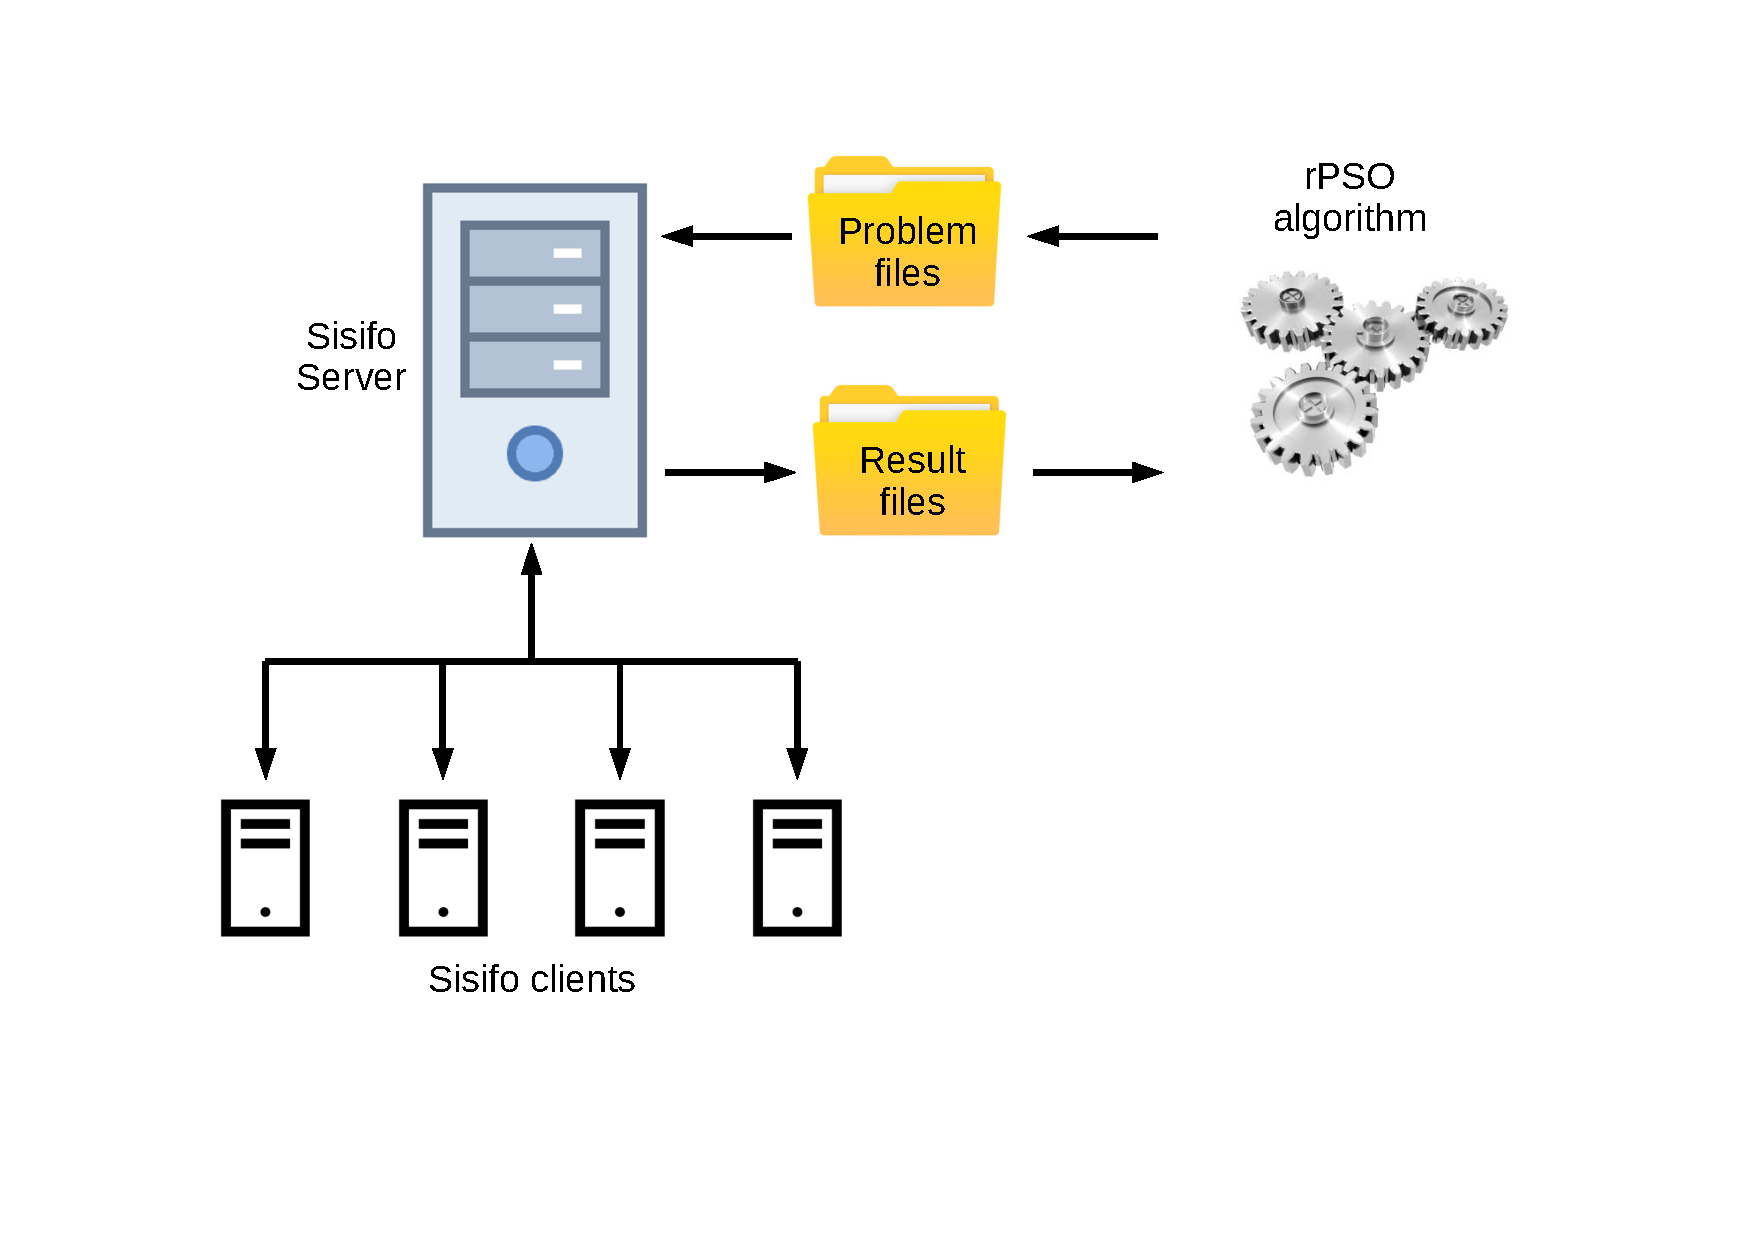
\includegraphics[width=0.6\linewidth]{IMGs/1.-Calibrado/Esquema_2.pdf}
	\caption{Introduction of the asynchronous rPSO algorithm in the Sisifo environment. rPSO manages the generation of new problems and put them in the \textit{Problem files} folder and the reading and processing of the solution files located in the \textit{Result  files} folder.}
	\label{rPSO.python}
\end{figure}

When the procedure starts running, with the initialization of the particles (Step 1) we create their corresponding problem files in the \textit{Problem files} folder. The \textit{Sisifo Server} detects new problem files and distribute them among idle \textit{Sisifo Clients}. These clients carry out the realizations. When a Sisifo client ends its task, a results file is generated and sent to the \textit{Sisifo Server} that drops it on the \textit{Result files} folder. Every time a new results file appears in the \textit{Results files} folder, the asynchronous rPSO, in Step 4, reads the data from the results file and calculates the fitness. Then, updates the velocity taking into account the current existing global best and its individual best particles (Step 2), updates the particle (Step 3) and with the new model parameters creates a new problem file in the \textit{Problem files} folder. And so on. 

\subsubsection{Fitness function and some features included in the rPSO}\label{sec:rPSO}
There are some features included in our version of the asynchronous rPSO algorithm that we have to describe. 

\begin{enumerate}
	\item In the Step 3, we include the possibility to discard the new particle and generate a new one randomly with $10\%$ probability. If it is not discarded, with $10\%$ probability we apply to the new particle a mutation.  
	\item The fitness evaluation is made as follows: 
	\begin{itemize}
		\item we start the model and after a warm-up time of $ 400 $ simulated months, we get a stabilization of the model output; 
		\item we take the model output from month $ 401 $ to $ 500 $ for the subpopulations in the data of Table \ref{datos}, i.e., percentage of women HR- and LR-infected per group ages $18-29$ and $18-64$;  
		\item then, for each subpopulation, we calculate the maximum and the minimum of these portions of the model output and we see if these maximum and minimum are inside the corresponding data $95\%$ confidence interval;
		\item if this happens, the fitness is zero; 
		\item otherwise, the fitness is the sum of the distances from these maxima and minima to the corresponding $95\%$ confidence interval of the data.
	\end{itemize}
	
	\item The definition of the fitness function may provide the same fitness values for different particles. Therefore, we are going to store all the particles with the same best fitness and, in Step 2, we chose  $p_{global}^{best}$ randomly among the stored particles.	
	\item As we mentioned before, physicians around the world have published estimations of most of the model parameters \cite{Durex2002,elbasha2007model,Giuliano2011,Nyitray2015}. It is clear that we have to respect their estimation in our fitting procedure avoiding that some model parameters overpass the estimation intervals. Furthermore, finding model parameters in the range of the estimations, gives credibility to our model. Therefore, when a model parameter is less than $1\%$ closer to an extreme of the interval provided by the physician estimations, we discard this value and it is substituted by a random value inside the interval.  
\end{enumerate}

It is worth to note that the above points 1, 3 and 4 will allow us to explore extensively the whole space of parameters avoiding the accumulation of particles close to the borders. 

\begin{remark}\label{mo}
At this point, we want to remark that to evaluate the fitness function, we do not need the model output for all the subpopulations. Only is necessary the output corresponding to HR- and LR-infected women in the group ages $18-29$ and $18-64$. Then, when a realization is carried out, we retrieve and process from the results file the data corresponding to the above subpopulations from the month $401$ to $500$, write them in a row and this row is stored as the result of the realization to be used later. 

Also, in order to compare properly the model output row with the data, we build the data vector mean, percentile $2.5$ and percentile $97.5$, repeating $100$ times the $4$ values of each we have in the Table \ref{datos} and write them in a row.
\end{remark}

\subsection{Selecting an optimal number of particles to calibrate the HPV large network computational model with rPSO}
As we have mentioned above, on previous implementations of the parallel rPSO, we realized that we can not affirm that \textit{the higher the number of particles, the better the quality of the solution}. Moreover, we also detected that, due to our asynchronous parallel implementation, sometimes the use of more processors does not mean lower execution times. We would need more experiments to detect the correct cause of the delays. However, in this case is more practical to investigate what the optimal combination of particles is to achieve the best quality with the lowest number of processors.

To perform this test, we are going to build HPV network models with $50,000$ nodes. We run 5 repetitions of the same problem with different number of particles. Times are shown in seconds. Thus, the question is, what is the quality of the solutions for different number of particles? Table \ref{tab.color} shows relevant information regarding the quality of the solutions for different number of particles and 5 runs of each configuration. Each run carried out 1200 particle evaluations. We measure the quality of the solutions on Table \ref{tab.color} by counting the number of fitness values equal to zero in the 5 runs (\textit{Total \# 0s}) and on average (\textit{Avg \#0s}). In addition, we also recorded the iteration at which the first zero appear on average (\textit{Avg  First}), from the last population of particles Fitness of the best, worst and average, averaged over five runs (\textit{Best at end}, \textit{Worst at end} and \textit{Avg at end}). And regarding executions time we show on Table  \ref{tab.color} information about the average total execution time for 1200 evaluations (\textit{Total Time}), the  worst execution time for one particle (\textit{Worst $t$}) and the best execution time for one particle (\textit{Best $t$}). Red color indicates the worst configuration, bold letters indicate the best and blue color the second best configuration.

\begin{table}[h]
	\centering
	\begin{tabular}{cccccccccc}
		\hline
		\cellcolor[HTML]{C0C0C0}\#       & Total   & Avg   & Avg     & Best    & Worst   & Avg  & Total   &       &                            \\
		\cellcolor[HTML]{C0C0C0} Part. &     \#0s & \#0s   &First  &  at end  & at end &at end & Time & Worst t  &          Best t                     \\ 
		\hline
		\cellcolor[HTML]{C0C0C0}25          & 18            & {\color[HTML]{3166FF} 3.60} & \textbf{531.00}                & \textbf{0.015486}               & \textbf{0.429090}               & \textbf{0.122573}               & 8422.00                         & \textbf{148.60}                & \textbf{107.00}               \\
		\cellcolor[HTML]{C0C0C0}30          & \textbf{28}           & \textbf{5.60}               & {\color[HTML]{3166FF} 594.00}  & {\color[HTML]{3166FF} 0.003785} & {\color[HTML]{3166FF} 0.445587} & {\color[HTML]{3166FF} 0.131193} & \textbf{6908.00}                & {\color[HTML]{3166FF} 186.60}  & {\color[HTML]{3166FF} 112.00} \\
		\cellcolor[HTML]{C0C0C0}35          & 8             & 1.60                        & 834.80                         & 0.010211                        & 0.576688                        & 0.149215                        & {\color[HTML]{3166FF} 7105.00}  & 250.60                         & 119.60                        \\
		\cellcolor[HTML]{C0C0C0}40          & 16            & 3.20                        & 692.80                         & 0.003332                        & 0.524417                        & 0.132628                        & 8808.60                         & 389.40                         & 144.60                        \\
		\cellcolor[HTML]{C0C0C0}45          & 14            & 2.80                        & 790.40                         & 0.006458                        & 0.639775                        & {\color[HTML]{FE0000} 0.149670} & 10004.00                        & 502.00                         & 177.20                        \\
		\cellcolor[HTML]{C0C0C0}50          & 11            & 2.20                        & 796.00                         & {\color[HTML]{FE0000} 0.005168} & {\color[HTML]{FE0000} 0.658020} & 0.139089                        & 11124.40                        & 648.40                         & 220.00                        \\
		\cellcolor[HTML]{C0C0C0}55          & 2             & {\color[HTML]{FE0000} 0.40} & {\color[HTML]{FE0000} 1171.20} & 0.004330                        & 0.518894                        & 0.137088                        & 11905.80                        & 775.00                         & 207.40                        \\
		\cellcolor[HTML]{C0C0C0}60          & 12            & 2.40                        & 765.00                         & 0.002153                        & 0.546259                        & 0.132464                        & 13787.80                        & 857.00                         & 245.40                        \\
		\cellcolor[HTML]{C0C0C0}64          & 5             & 1.00                        & 985.40                         & 0.002763                        & 0.551228                        & 0.140977                        & {\color[HTML]{FE0000} 18770.00} & {\color[HTML]{FE0000} 1041.20} & {\color[HTML]{FE0000} 379.20} \\ \hline
	\end{tabular}
	\caption{Analysis of the quality and execution times of different rPSO configurations. Results of 1200 evaluations for different number of particles on the rPSO process (\# Part.).}
	\label{tab.color}
\end{table}

As we can see, 25 and 30 particles are the preferred configurations, since we obtained the higher number of zeros in total and on average and the lower executions times. Since the results of 25 particles shows a very good run with 7 zeros and also a very good execution time, we can conclude that the configuration with 30 particles should be selected bearing in mind both quality and execution time. Results on total number of 0s and total time were statically significant with $p$ value of $0.1$ after an ANOVA analysis.

\subsection{Improving the exploration of the rPSO}
As we explained on Section \ref{sec:rPSO}, we established a procedure respect to the intervals for the parameter values proposed by physicians. Some algorithms such as differential evolution \cite{storn1997differential} allows to overpass these limits in the search of a good combination of parameters. However, this is not a good idea when implementing our parallel rPSO. First, remember that our parallel version is asynchronous and the updating of the particles is made once every particle is evaluated. Allowing particles with parameters close to the limits trespass them, could lead to a chaotic search. Second, parameters out the defined bounds have not a medical meaning. Therefore, when a model parameter is less than $1\%$ closer to an extreme of the interval provided by the  estimations, we discard this value and it is substituted by a random value inside the interval. This allows also to made a deeper and more efficient exploration of the search space.

Figures in Table \ref{Ctg} show the exploration performed in some of the parameters of the model (duration and contagion parameters). Figures represent the values of the parameters during the 20 executions of rPSO algorithm with 500 realizations each one. X axis represents the realization number and Y axis the value of each parameter. We can see that we find points on most of the search space.

\begin{table}[!h]
\begin{center}	
\begin{tabular}{cc}
	Time of clearance of HPV high risk & Time of clearance of HPV low risk \\
	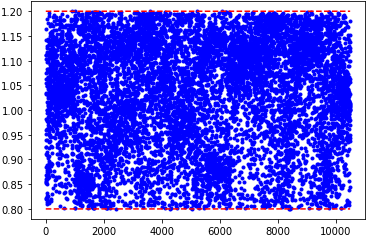
\includegraphics[width=0.4\textwidth]{IMGs/1.-Calibrado/Dura_HR_H.png} & 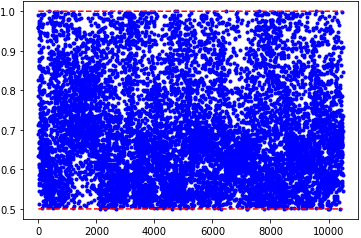
\includegraphics[width=0.4\textwidth]{IMGs/1.-Calibrado/Dura_LR_H.png} \\ 
	\\
	Women transmission probability of HPV low risk & Men transmission probability of HPV high risk \\
	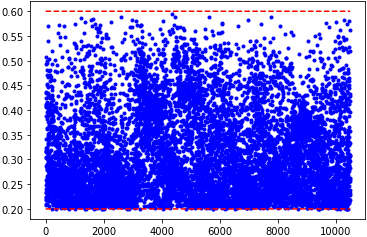
\includegraphics[width=0.4\textwidth]{IMGs/1.-Calibrado/Ctg_M_LR.png} & 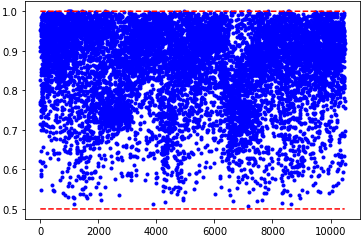
\includegraphics[width=0.4\textwidth]{IMGs/1.-Calibrado/Ctg_H_HR.png}  
\end{tabular}
\caption{Upper figures: Time of clearance of HPV high risk and low risk, both for men and women. Lower figures: on the left, probability to transmit low risk HPV if the infected is a woman; on the right, probability to transmit high risk HPV if the infected is a man. Red dashed lines correspond to the bounds of each parameter. We can see that most of the search space is explored in all the cases.} 
\label{Ctg}
\end{center}
\end{table}

\subsection{Calibrating the model}
Now, we are going to perform the calibration. We use the Sisifo environment with the modified rPSO and 30 particles. The HPV network models will have $100,000$ million nodes. In order to guarantee the reproducibility of the realizations, we are going to include in the problem files and store seeds for the generation of the random numbers during the calibration process.

We assume that, initially, data of prevalence from Table \ref{datos} are not only for women but also for men. Then, we label women and men as infected randomly following these prevalence data. Also, we start running the realization and the first $400$ months are used as a warm-up period to stabilize the distribution of infected men and women. Thus, the goal is to calibrate the model parameters in such a way that the model output related to women HR and LR prevalence minimize the fitting function defined in Section \ref{sec:rPSO}.

We have performed 20 different calibrations using rPSO, each one with around $500$ realizations and $30$ particles. A total of $10,100$ realizations of the model were performed with an equivalent sequential total computation time of $161$ days.

\begin{figure}[h!]
	\centering
	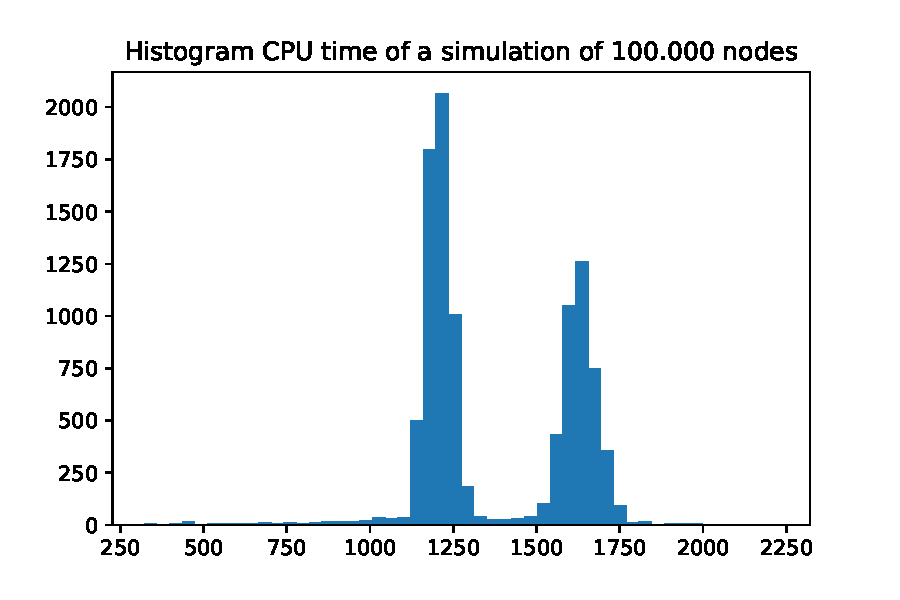
\includegraphics[width=0.6\linewidth]{IMGs/1.-Calibrado/Hist_CPU_time.pdf}
	\caption{Histogram of the computation time of each one of the $10,100$ realizations of the model using networks of $100,000$ nodes. The average time is $1374.5$ seconds, around $23$ minutes.}
\end{figure}

\subsection{Selecting the 30 realizations that best capture the data uncertainty}
Our goal, now, is to find a procedure to select $30$ among the $10,100$ realizations of the model in such a way that the means and the 95\% confidence intervals of these $30$ realizations be as much close as possible of the corresponding means and the 95\% confidence intervals of the data in Table \ref{datos}. We decided to select $30$ because as we saw in Table \ref{tab.color}, the total computation time is the best for $30$ particles running in parallel in the Sandy Bridge computer.

Nevertheless, it would be interesting to reduce the number of eligible realizations to much less than $10,100$. In Figure \ref{Error_0} we can see the $100$ realizations with error less than $0.01$, that is, the realizations that almost lie inside the 95\% confidence intervals of the data, represented by the blue horizontal dashed lines. If we select $30$ among these $100$, it is clear that some percentiles of the model will be far from the corresponding percentiles of the data, for instance, the lower parts of the left figures. Therefore, we need to consider realizations with errors greater than $0.01$ without forgetting the objective to reduce the number of eligible realizations.  

\begin{figure}[h!]
	\centering
	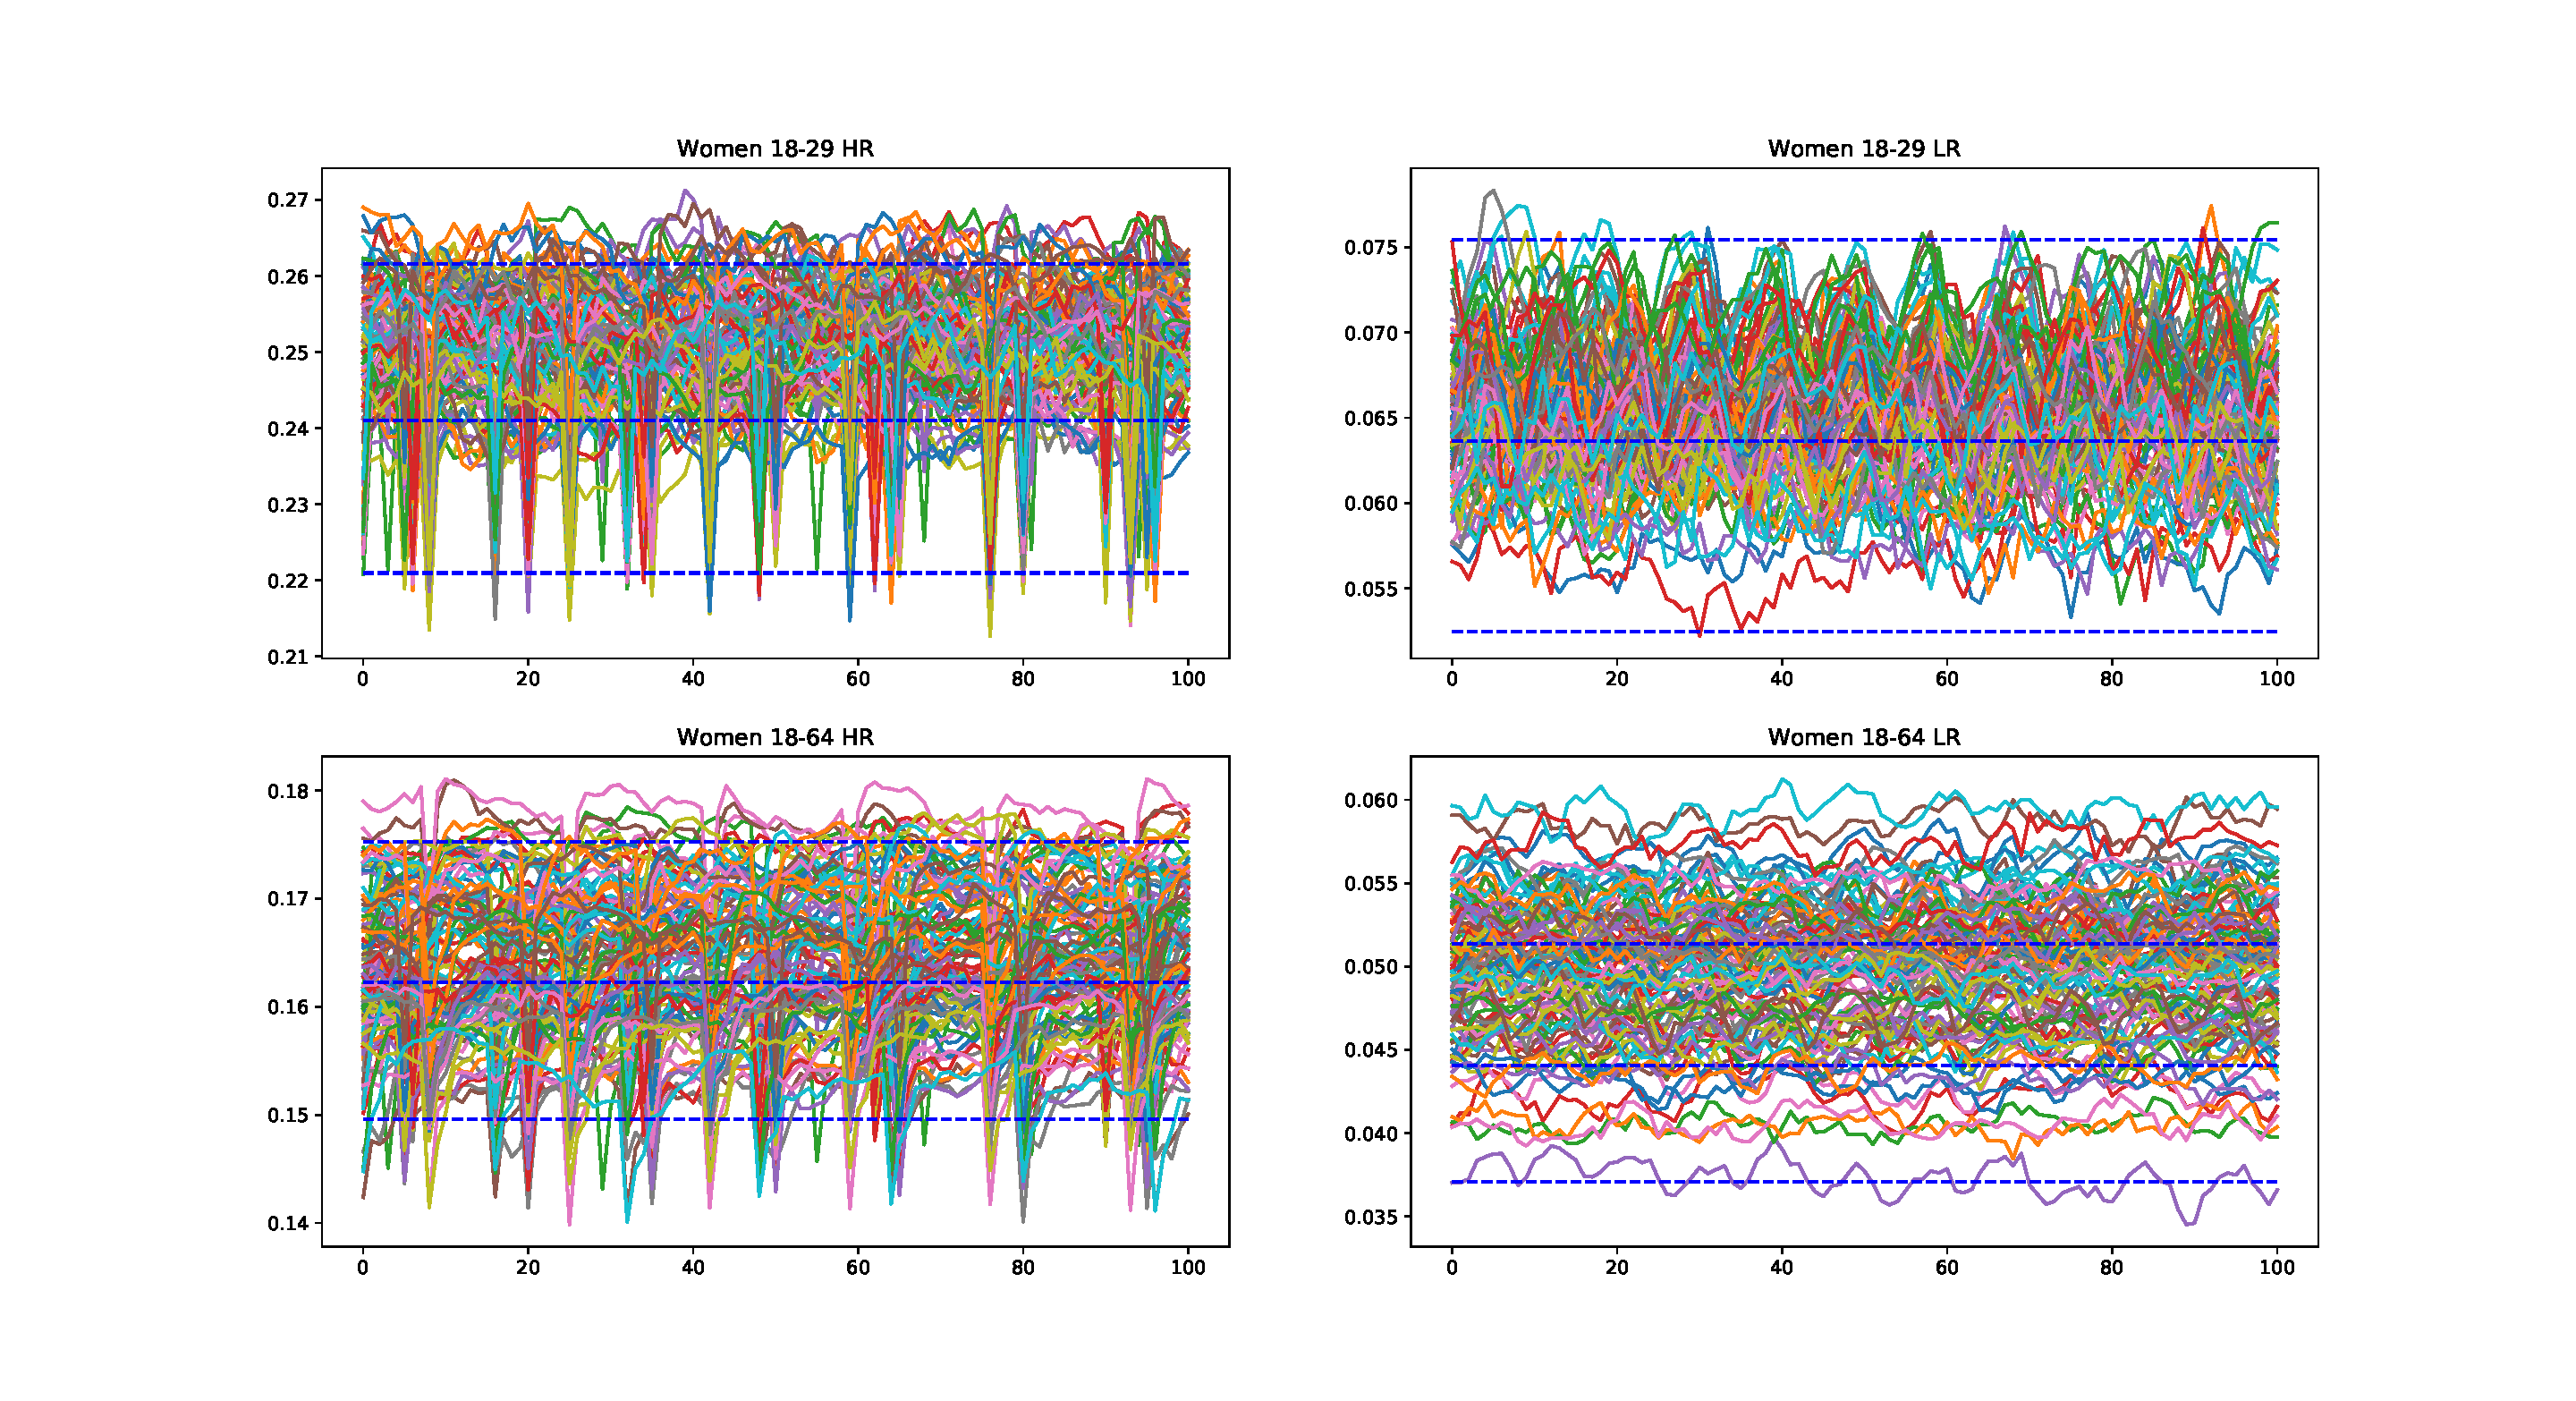
\includegraphics[width=\linewidth]{IMGs/1.-Calibrado/Error_001.pdf}
	\caption{Drawing of the $100$ model realizations with error less than $0.01$ from month 400 to 499. }
	\label{Error_0}
\end{figure}

Thus, we check the number of possible realizations depending on their error. Then, there are $2$ realizations with error $0$,  $100$ realizations with error less than $0.01$, $392$ with error less than $0.025$, $1282$ with error less than $0.05$ and $2607$ with error less than $0.075$. In Figure \ref{Error_003}, we draw the $1282$ model realizations of with error less than $0.05$. Note that the realizations cover completely the 95\% confidence intervals of the data. 

\begin{figure}[h!]
	\centering
	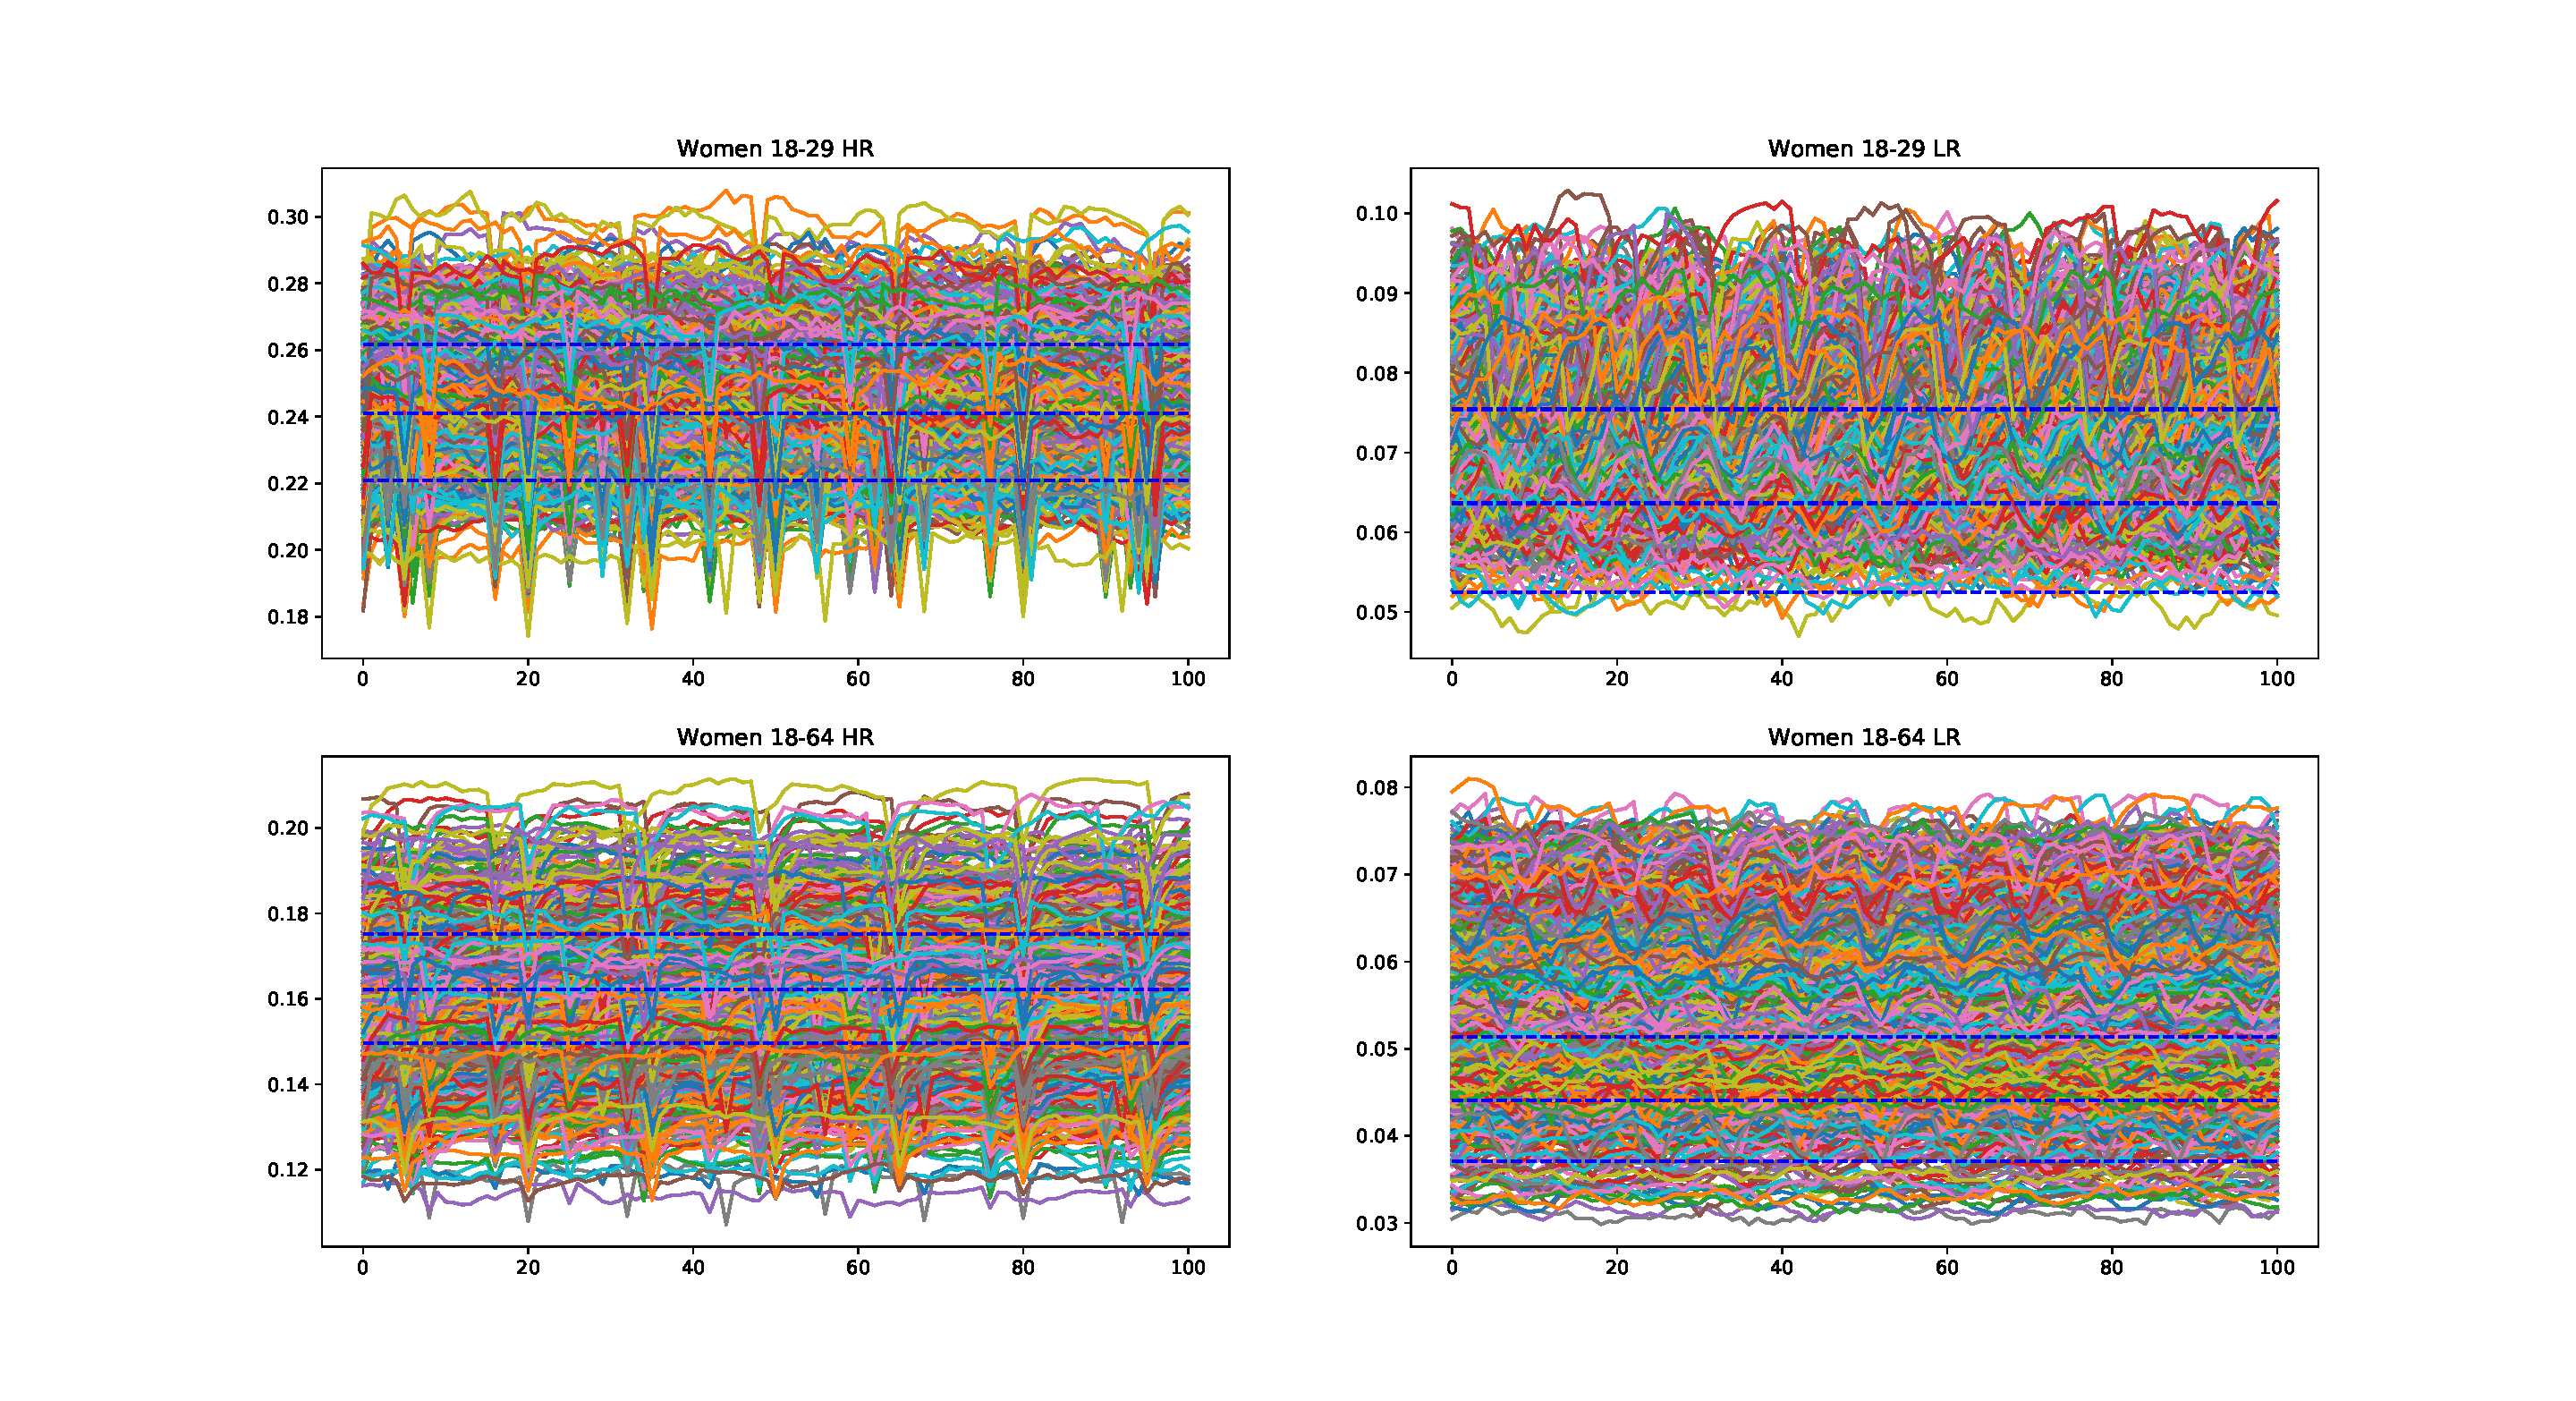
\includegraphics[width=\linewidth]{IMGs/1.-Calibrado/Error_005.pdf}
	\caption{Drawing of the $1282$ model realizations with error less than $0.05$ from month 400 to 499. These realizations cover the 95\% confidence intervals of the data, represented by the blue horizontal dashed lines.}
	\label{Error_003}
\end{figure}

In order to determine the \textit{best} $30$ realizations that capture the mean and the $95\%$ confidence intervals of the data in Table \ref{datos}, we are going to introduce an adapted version of the rPSO algorithm before. Let $E$ be the realizations considered with $card(E)=M$ its number. For instance, for $E$ the set of realizations with error less than $0.01$, $M=100$. Also, for $E$ the set of realizations with error less that $0.05$, $M=1282$. Then $E(i)$ is the $i-th$ realization of the set $E$. We define the following fitness function $F$:

\begin{description}
	\item[INPUT:] Set of $30$ indexes $I=\{i_1,\ldots,i_{30} \}$, $1\leq i_j \leq M$, $j=1,\ldots, 30$..
	\item[Step 1.] Select the realizations $E(i_1),\ldots,E(i_{30})$ and calculate the mean, percentile $2.5$ and percentile $97.5$ of them.
	\item[Step 2.] Calculate the norm of the difference between the mean, percentile $2.5$ and percentile $97.5$  of the $30$ realizations and the data (see Remark \ref{mo}), and sum them up. 
\end{description}

Now, the adapted version of rPSO to select the best $30$ realizations is

\begin{description}
	\item[Step 1.] Initialization.
	\begin{itemize}
		\item We have a set $E$ with $M$ realizations.
		\item Initialize $N$ index subsets $S_1,\ldots,S_N$ with $30$ elements of the set $\{1,\ldots,M\}$ (particles) chosen randomly without repetition.
		\item Evaluate the fitness of all the particles $F(S_1), \ldots, F(S_N)$.
		\item Define the individual best fitness as $S_i^{best} = S_i$, $i=1,\ldots,N$ and the global best fitness $S_{global}^{best}$ as the $S_i^{best}$ which fitness is the minimum.
	\end{itemize}
	\item[Step 2.] For $i=1,\ldots,N$, build the new set $P_i=S_i \cup S_i^{best} \cup S_{global}$, that is, joining the current particle, its individual best and the global best. After removing index repetitions, the new particle $S_i$ consists of a random selection without repetition of $30$ indexes of $P_i$.
	\item[Step 3.] Evaluate the fitness of all the new particles $F(S_1), \ldots, F(S_N)$.	
	\item[Step 4.] Update the individual best fitnesses $S_i^{best} = p_i$, $i=1,\ldots,N$ and  the global best fitness $S_{global}^{best}$. Go to Step 2. 
\end{description}

Here, we also consider $10\%$ of randomness and $10\%$ of mutation when updating new particles. In this case, mutation consists of changing some of the indexes in the current particle by other randomly chosen indexes, avoiding repetitions.

The above algorithm, in the tests we have run, lasts around $20$ minutes for $1$ million of evaluations of the fitness function in the Sandy Bridge computer, returning accurate solutions.

We have performed runs for $30$, $40$, $50$ and $60$ particles, being $E$ the realization sets with errors less than $0.025$, $0.05$ and $0.075$. The lowest error has been $0.1166$ for the following realizations  

\begin{equation}
\begin{array}{c}
85, 109, 460, 474, 475, 476, 485, 493, 496, 497, 523, 531, 542, 543, 563, 600, \\
635, 637, 650, 687, 715, 729, 730, 842, 974, 987, 1058, 1060, 1080, 1238,	
\end{array}
\label{laselegidas}    
\end{equation}

among the $1282$ of the set of realizations with error less than $0.05$. In Figure \ref{fig:laselegidas} we draw the selected realizations and in Figure \ref{fig:ajuste95IC} we can see the graphical result of the calibration and how resemble the means and 95\% confidence intervals.  

\begin{figure}[h!]
	\centering
	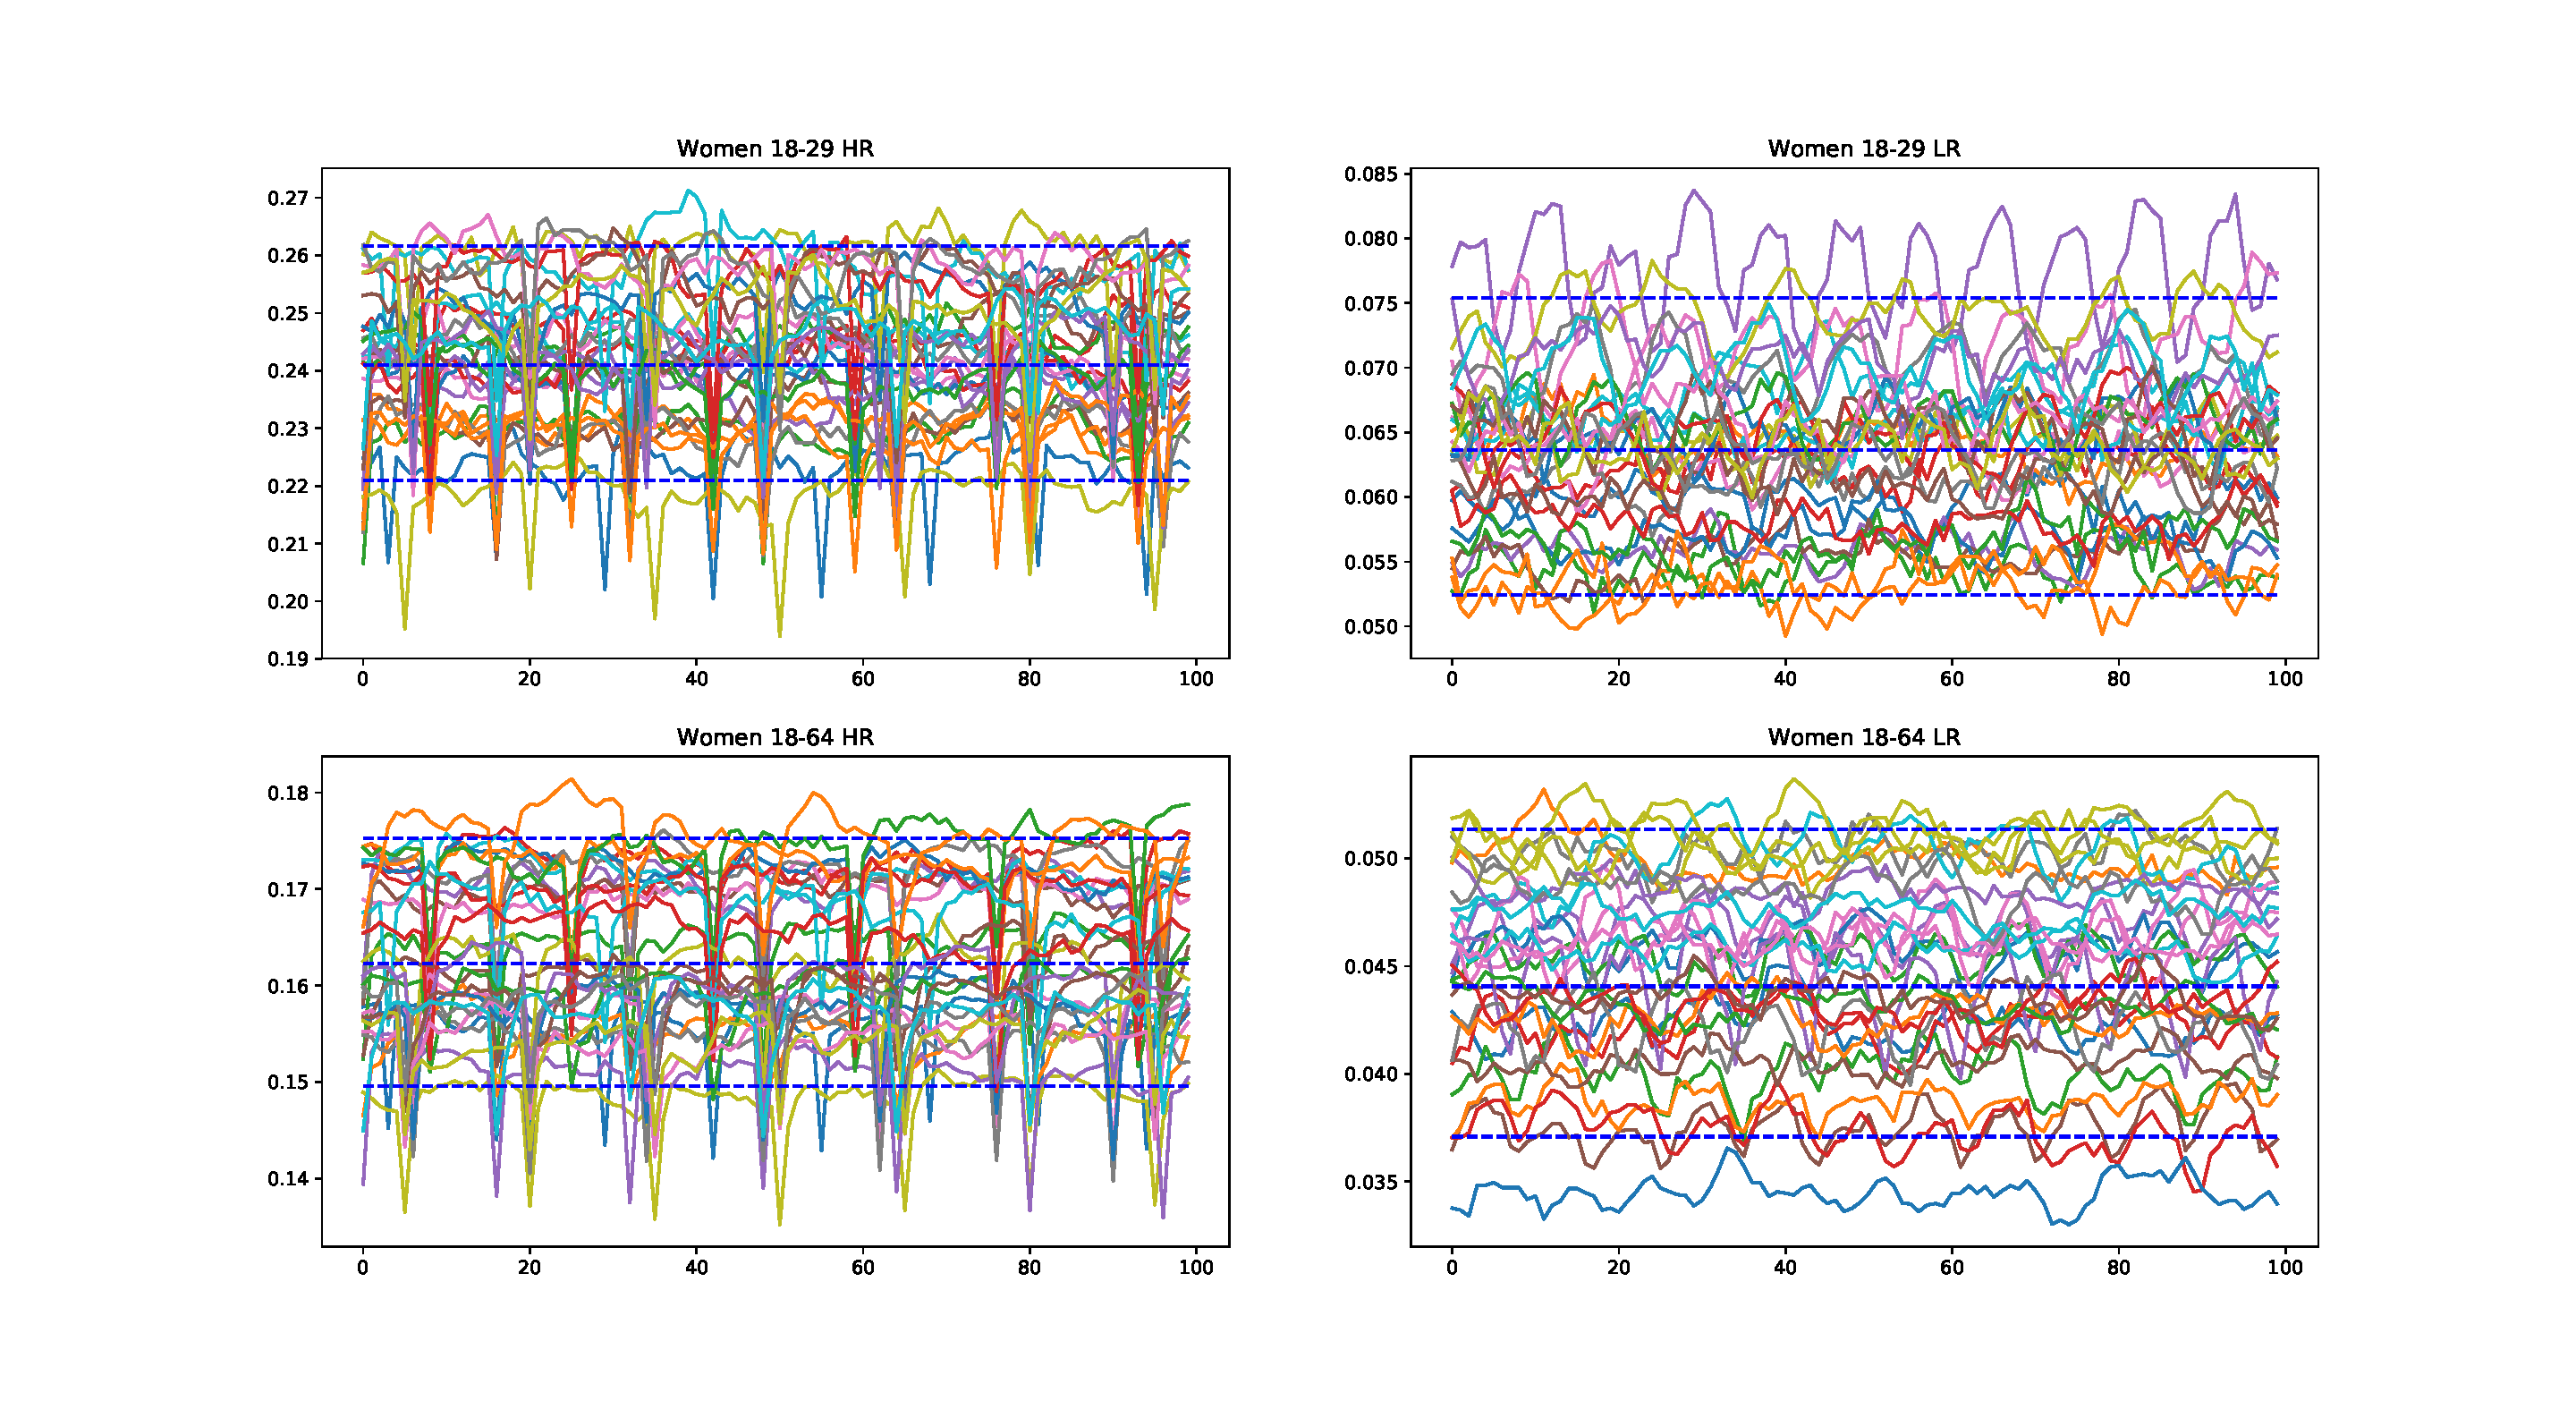
\includegraphics[width=\linewidth]{IMGs/1.-Calibrado/Selected.pdf}
	\caption{Drawing of the $30$ selected model realizations from month 400 to 499. These realizations are the ones whose means and 95\% confidence intervals resemble the most the data in Table \ref{datos}, represented by the blue horizontal dashed lines.}
	\label{fig:laselegidas}
\end{figure}

\begin{figure}[h!]
	\centering
	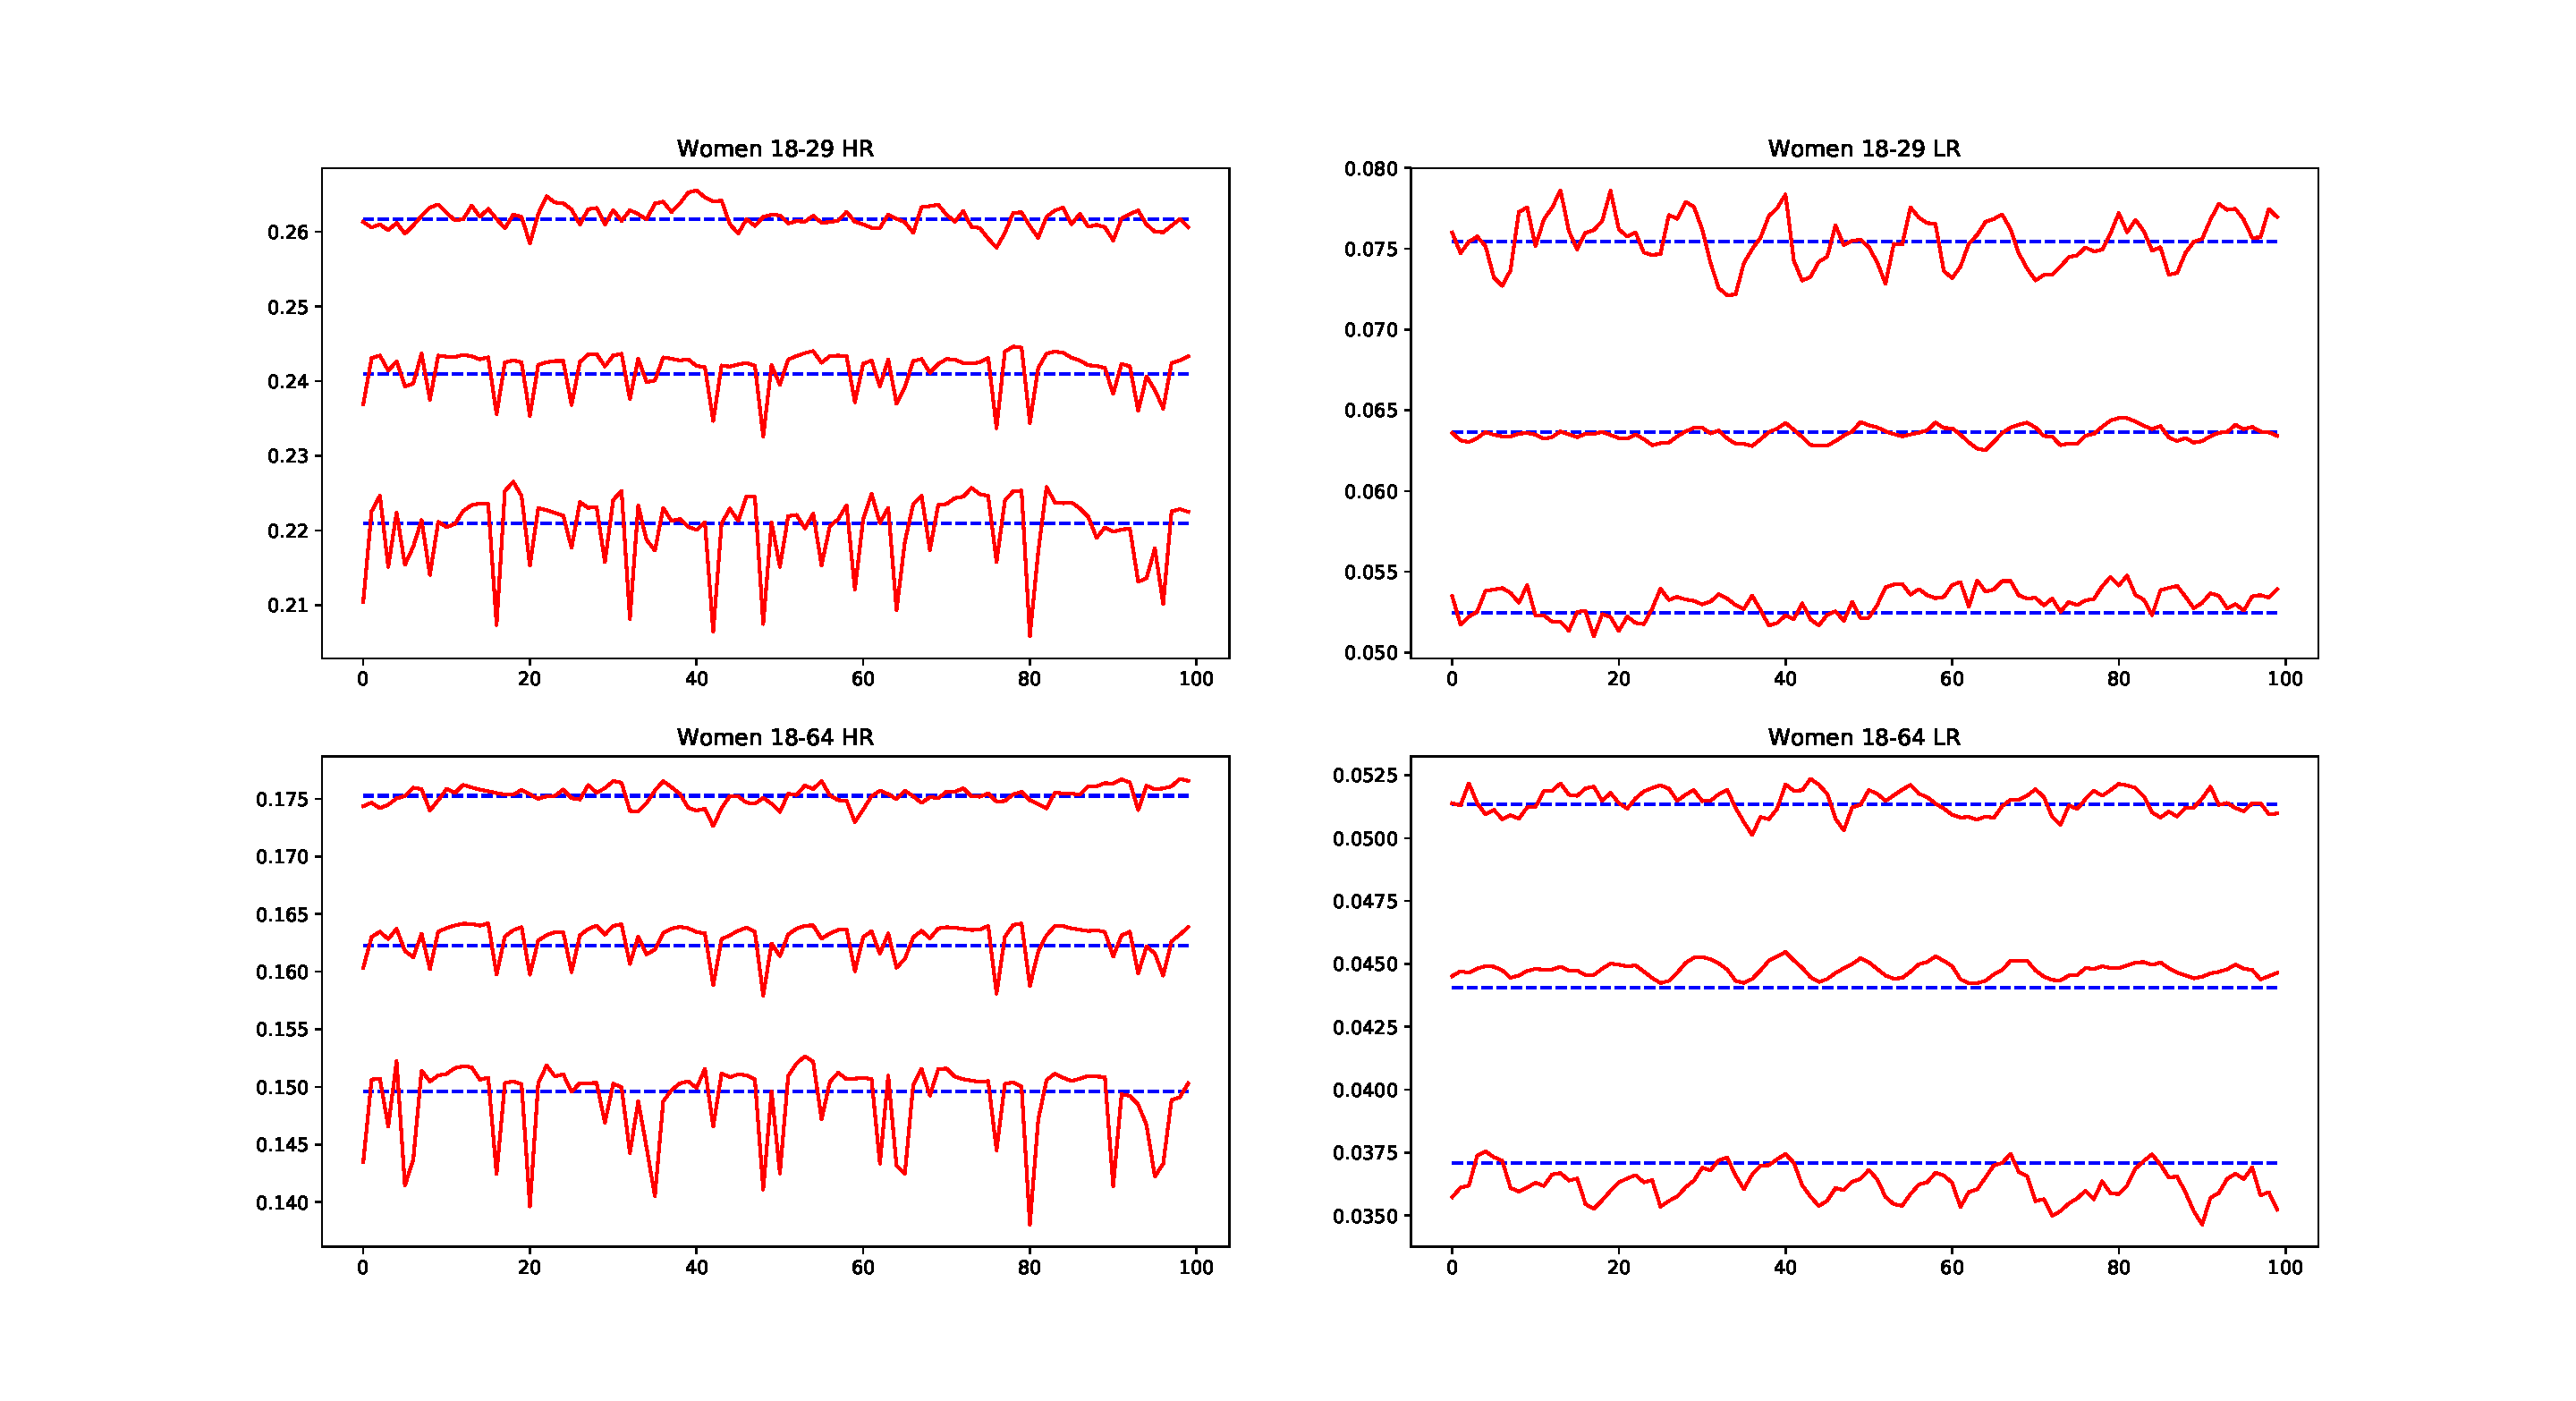
\includegraphics[width=\linewidth]{IMGs/1.-Calibrado/Ajuste_95IC.pdf}
	\caption{Means and 95\% confidence intervals of the $30$ selected realizations (in red) compared to the means and 95\% confidence intervals of the data (blue).}
	\label{fig:ajuste95IC}
\end{figure}

The mean and the 95\% confidence interval of the model parameters corresponding to the $30$ selected realizations from \eqref{laselegidas} are given in the Table \ref{table:laselegidas}. Note that the obtained model parameters are in accordance to the medical parameters appearing in the literature and collected in Section \ref{sec:modelo}. 

\begin{table}[!h]
	\begin{center}
		\begin{tabular}{|c|c|c|}
			\hline 
			Model parameter & Mean & $95\%$ confidence interval  \\ 
			\hline 
			Average LSP men & $8.63$ & $ [ 7.15 ,  9.86 ]$  \\ 
			Average time clearing HR HPV & $1.08$ &  $[ 0.88 ,  1.19 ]$ \\ 
			Average time clearing LR HPV &  $0.60$ & $ [ 0.52 ,  0.82 ]$\\ 
			Probability a woman transmits LR &  $0.23$ &  $[ 0.21 ,  0.29 ]$\\ 
			Probability a man transmits LR &  $0.28$ &  $[ 0.22 ,  0.37 ]$\\ 
			Probability a woman transmits HR &  $0.81$ & $[ 0.68 ,  0.95 ]$\\ 
			Probability a man transmits HR &  $0.91$ & $[ 0.74 ,  0.97 ]$ \\
			\hline
		\end{tabular}
	\end{center} 	
	\caption{Mean and the 95\% confidence interval of the model parameters corresponding to the $30$ selected realizations from \eqref{laselegidas}.}
	\label{table:laselegidas}
\end{table}
%GM_hom 7.890084666666667 , [ 7.055565249999999 ,  9.175369750000002 ]
%Dura_HR_H 1.0815233666666668 , [ 0.984595275 ,  1.1799214999999998 ]
%Dura_LR_M 0.6020232666666666 , [ 0.520799475 ,  0.7130141 ]
%Ctg_M_LR 0.24630120000000003 , [ 0.20750732500000002 ,  0.29335349999999993 ]
%Ctg_H_LR 0.2989984000000001 , [ 0.227862775 ,  0.38451014999999994 ]
%Ctg_M_HR 0.7533814333333333 , [ 0.5907493 ,  0.8939666999999999 ]
%Ctg_H_HR 0.8972156666666666 , [ 0.77310225 ,  0.9853232749999998 ]

In the following, we are going to use the sets of parameters corresponding to the realizations \eqref{laselegidas} (and their corresponding seeds) to perform the simulations below. 

%Cap�tulo 4 - dinamica y vacunacion del articulo Report HPV RJVM August 25, 2018
\chapter{Making Dynamic Sexual Contacts Network and adding Vaccination Campaigns}\label{DinamicaYVacunacion}
\section{Including new features into the model}
\subsection{Introducing age and LSP dynamics into the LSP model}
The computational model presented so far is static, that is, once we have assigned the LSPs, they do not change over the time and the nodes do not increase their age. We modulate the possibility of a contagion introducing global probabilities that determine if the existence of a LSP implies sexual intercourses in a given time step per age group $14-17$, $18-29$, $30-39$ and $40-65$. Also, note that the available data about LSPs come from $2003$ and the data of prevalence appears in a study (CLEOPATRA \cite{castellsague2012prevalence}) conducted in $2007-2008$. The sexual behavior has changed in the last $10-15$ years and we would like to include it in our model in some way. Nevertheless, newer data about LSPs and prevalence in Spain are not available.

Thus, in order to introduce age and LSP assignation dynamics in a simple way, we are going to \textit{move} the available data over the time. Figure \ref{fig:dinam1} shows the constant age distribution that do not varies over the time.

\begin{figure}[h!]
	\centering
	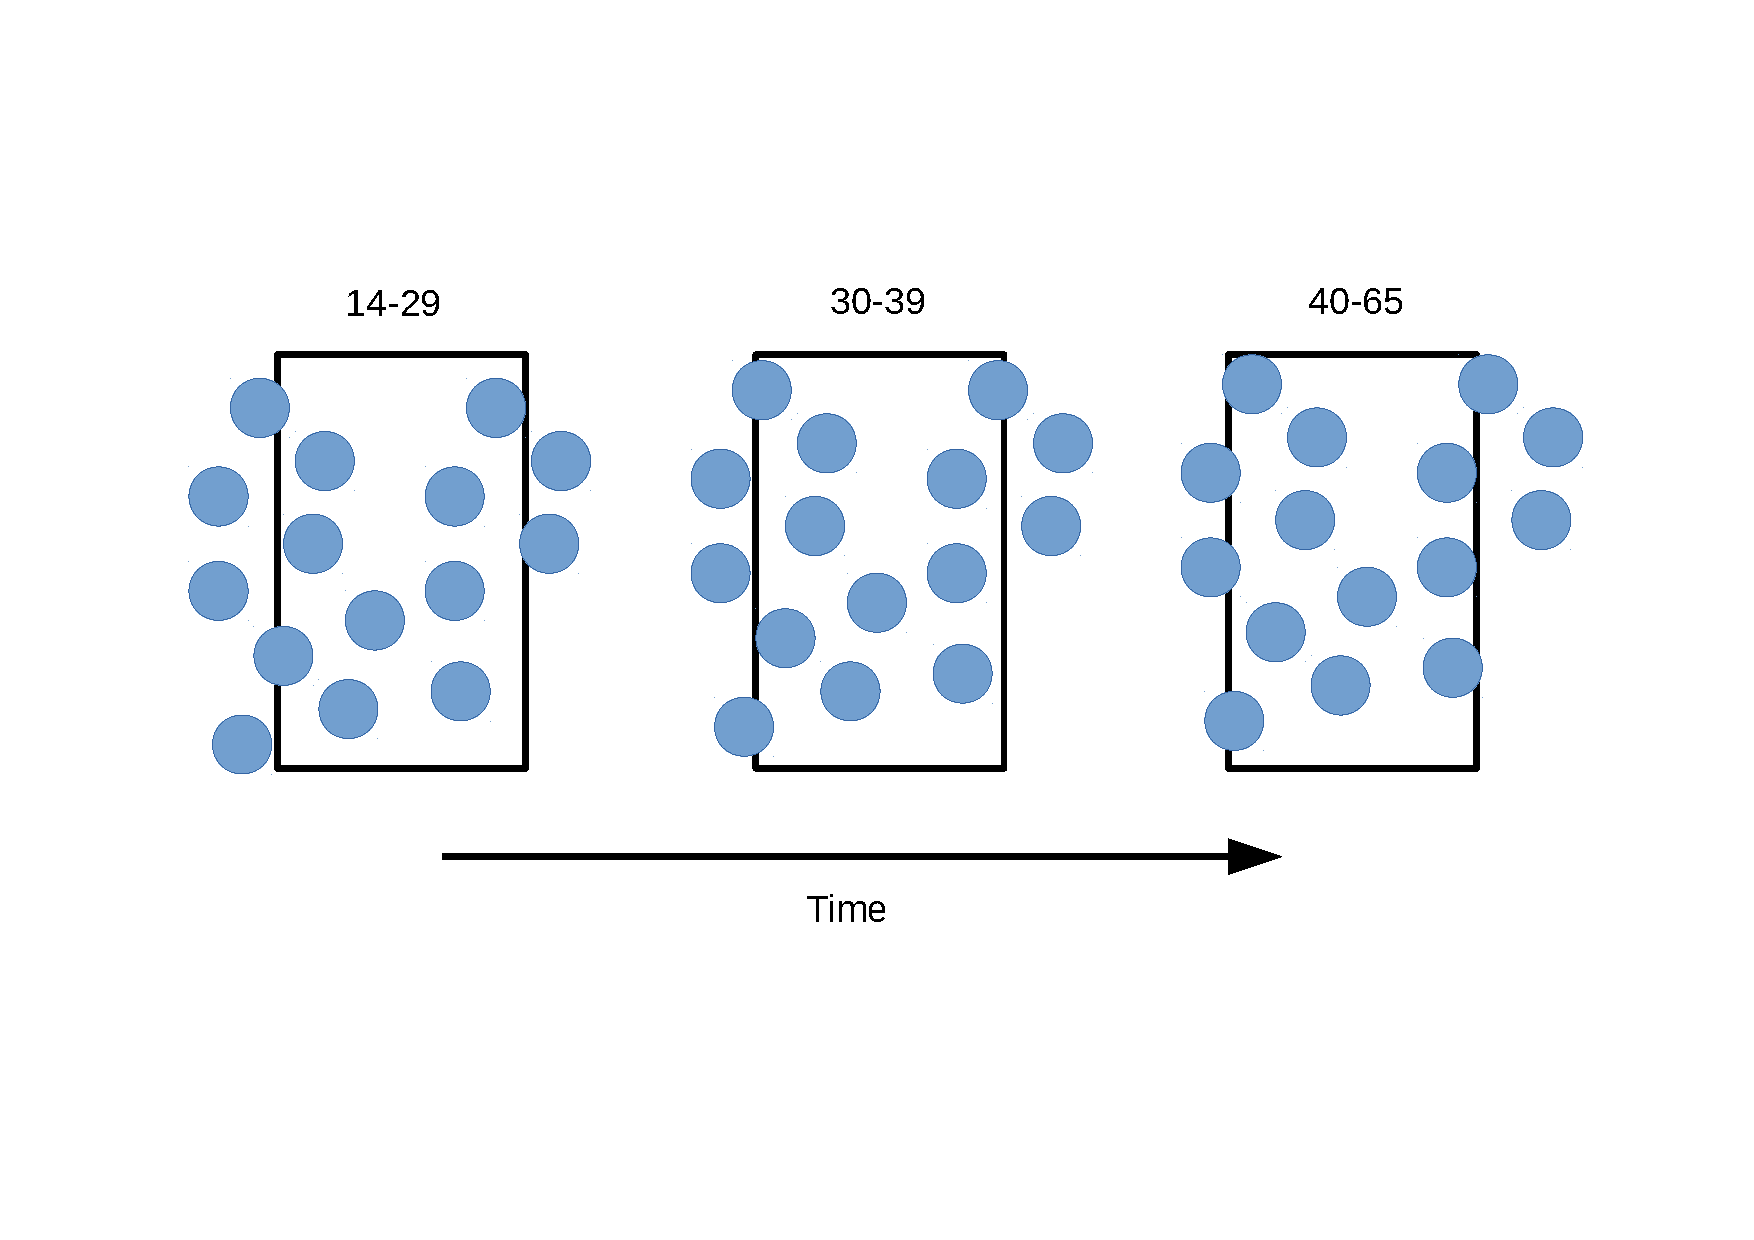
\includegraphics[width=0.7\linewidth]{IMGs/2.-New_features/Dinam_1.pdf}
	\caption{Static LSP network. The ages remain constant over the time. The time only affects the HPV contagion/clearing dynamics.}
	\label{fig:dinam1}
\end{figure}

Then, we evolve the ages of the nodes over the time. As long as the nodes do not change the age group, there is nothing to do. However, how do we \textit{recycle} the nodes that turn 65? And how do we transform the nodes in the first age group $14-29$ when they turn 30?  

To answer the first question, we propose to

\begin{itemize}
	\item preserve its sex in order to maintain the proportion males/females, 
	\item assign $14$ years old to the node, erase all its LSPs and transform it in susceptible,
	\item assign new LSPs according to the LSPs of the age group $14-29$ following the assortativity property.
\end{itemize}

To answer the second question, we propose to

\begin{itemize}
	\item preserve its sex and the infectious state, 
	\item erase all its LSPs and assign new LSPs according to the LSPs of the age group $30-39$ following the assortativity property.
\end{itemize}

This way, as time goes on, we will have the LSP structure by ages as we can see in the Figure \ref{fig:dinam2}.

\begin{figure}[h!]
	\centering
	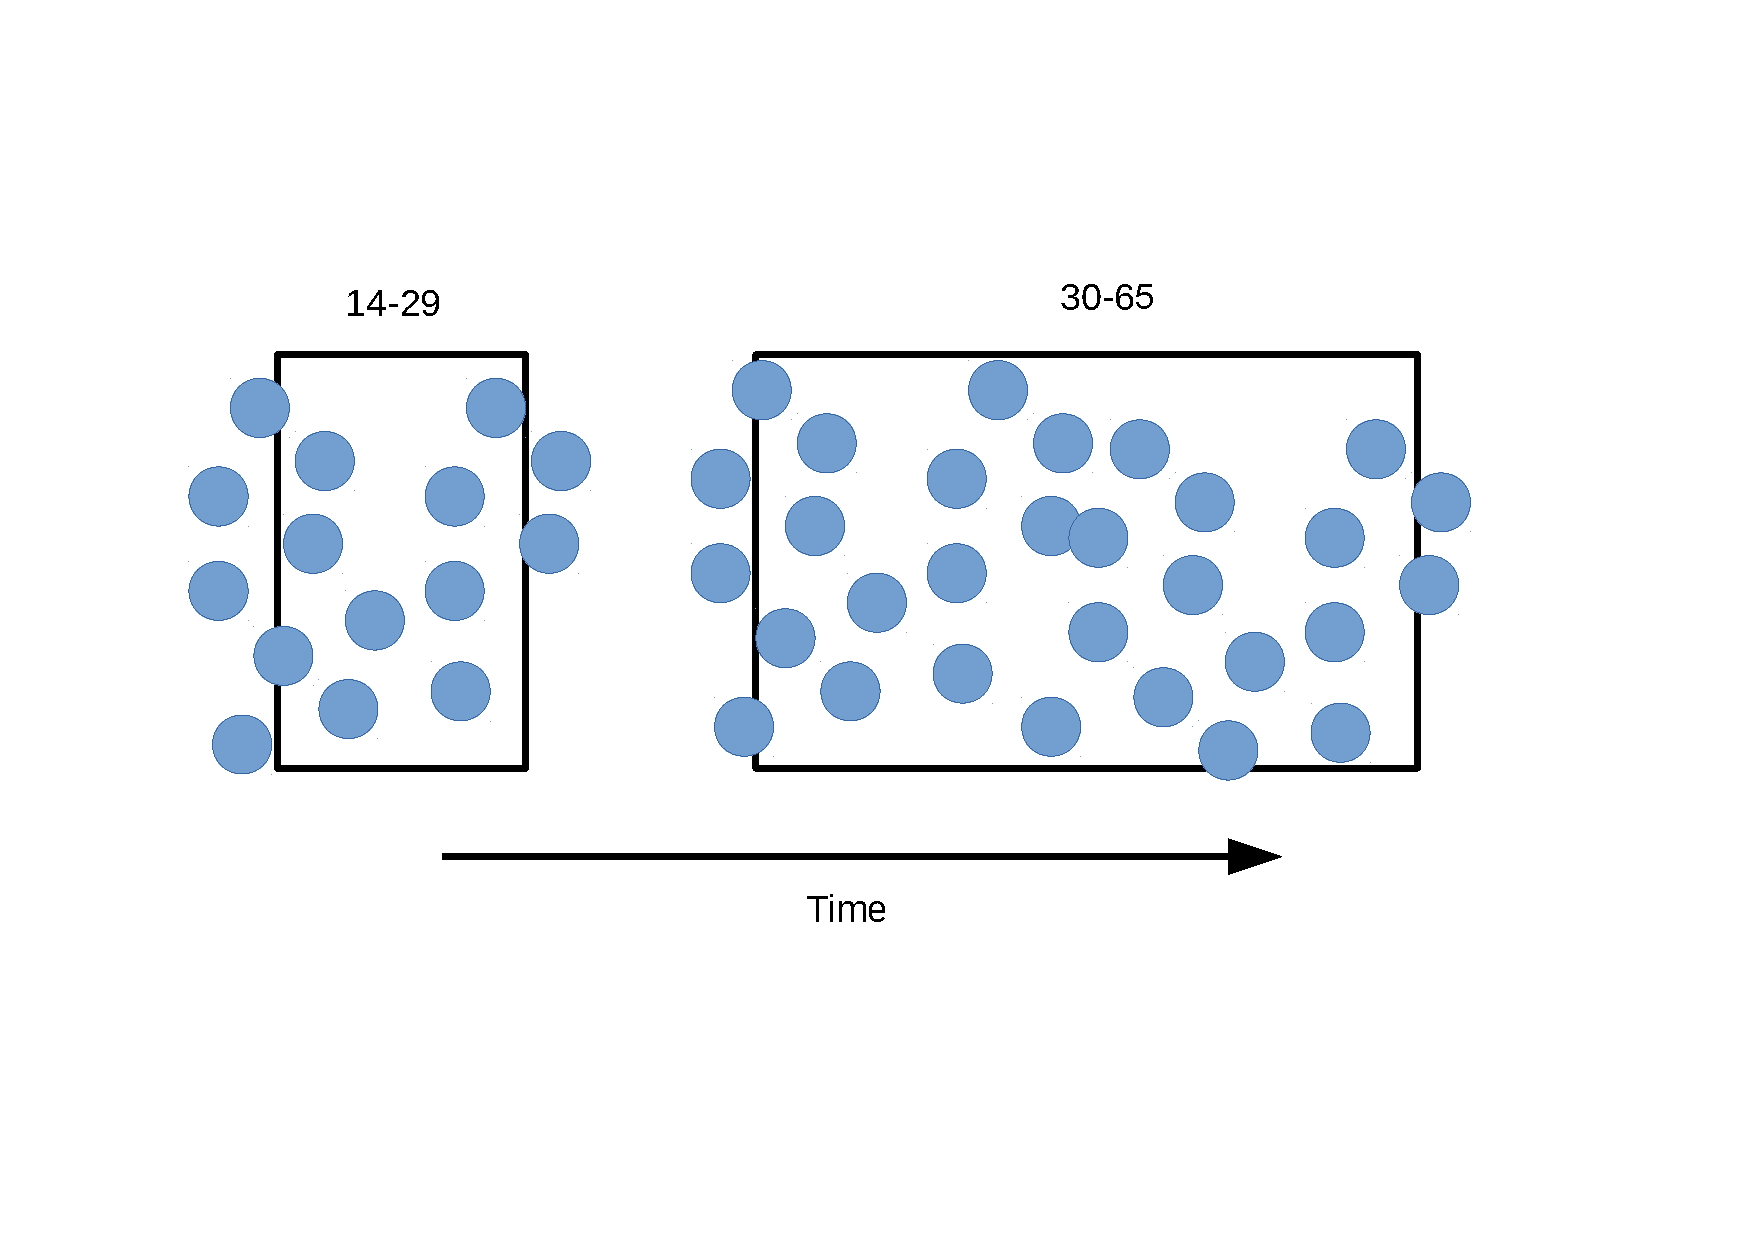
\includegraphics[width=0.7\linewidth]{IMGs/2.-New_features/Dinam_2.pdf}
	\caption{Dynamic LSP network. The ages evolve over the time. The age group 40-65 and their sexual behavior disappear when people grow.}
	\label{fig:dinam2}
\end{figure}

If the node is MSM (male who have sex with males), we perform the above procedure taking into account the division of age groups given in \cite{Durex2002}, $14-19$, $20-24$, $25-29$, $30-39$, $40-49$, $50-59$ and $60-64+$.

Taking into account that the global number of LSP in the age groups $40-65$ is less that in the age group $30-39$, as the time goes on, the global number of LSP in the whole network will increase and the transmission ot HPV will also increase. However, the proposed approach may be considered as very conservative because the sexual behavior change in the last $10-15$ years seems to result in an increase of the sexual intercourses greater than the number that we can approach with the proposed dynamic network. Nevertheless, the lack of data do not allow us to quantify the mentioned change.

%, but we take advantage of the static model building and the calibrated model parameters. Furthermore, as we mentioned before, we do not have recent data about sexual behavior in Spain.

\subsection{When should we start the vaccination schedule?} 
When a realization runs, we use $500$ months to stabilize the static network, then, we change to a dynamic network. Thus, a key point arises and it is to decide in which time instant starts the vaccination schedule. We have performed a simulation with the selected $30$ sets of parameters with $2300$ months (around $191.6$ years) where the network turns dynamic from the month $500$. In the Figure \ref{fig:Estudio_ciclos} we can see the levels of prevalence predicted by the model for 18-64 years old men and women for HR and LR, over the next years.

\begin{figure}[h!]
	\centering
	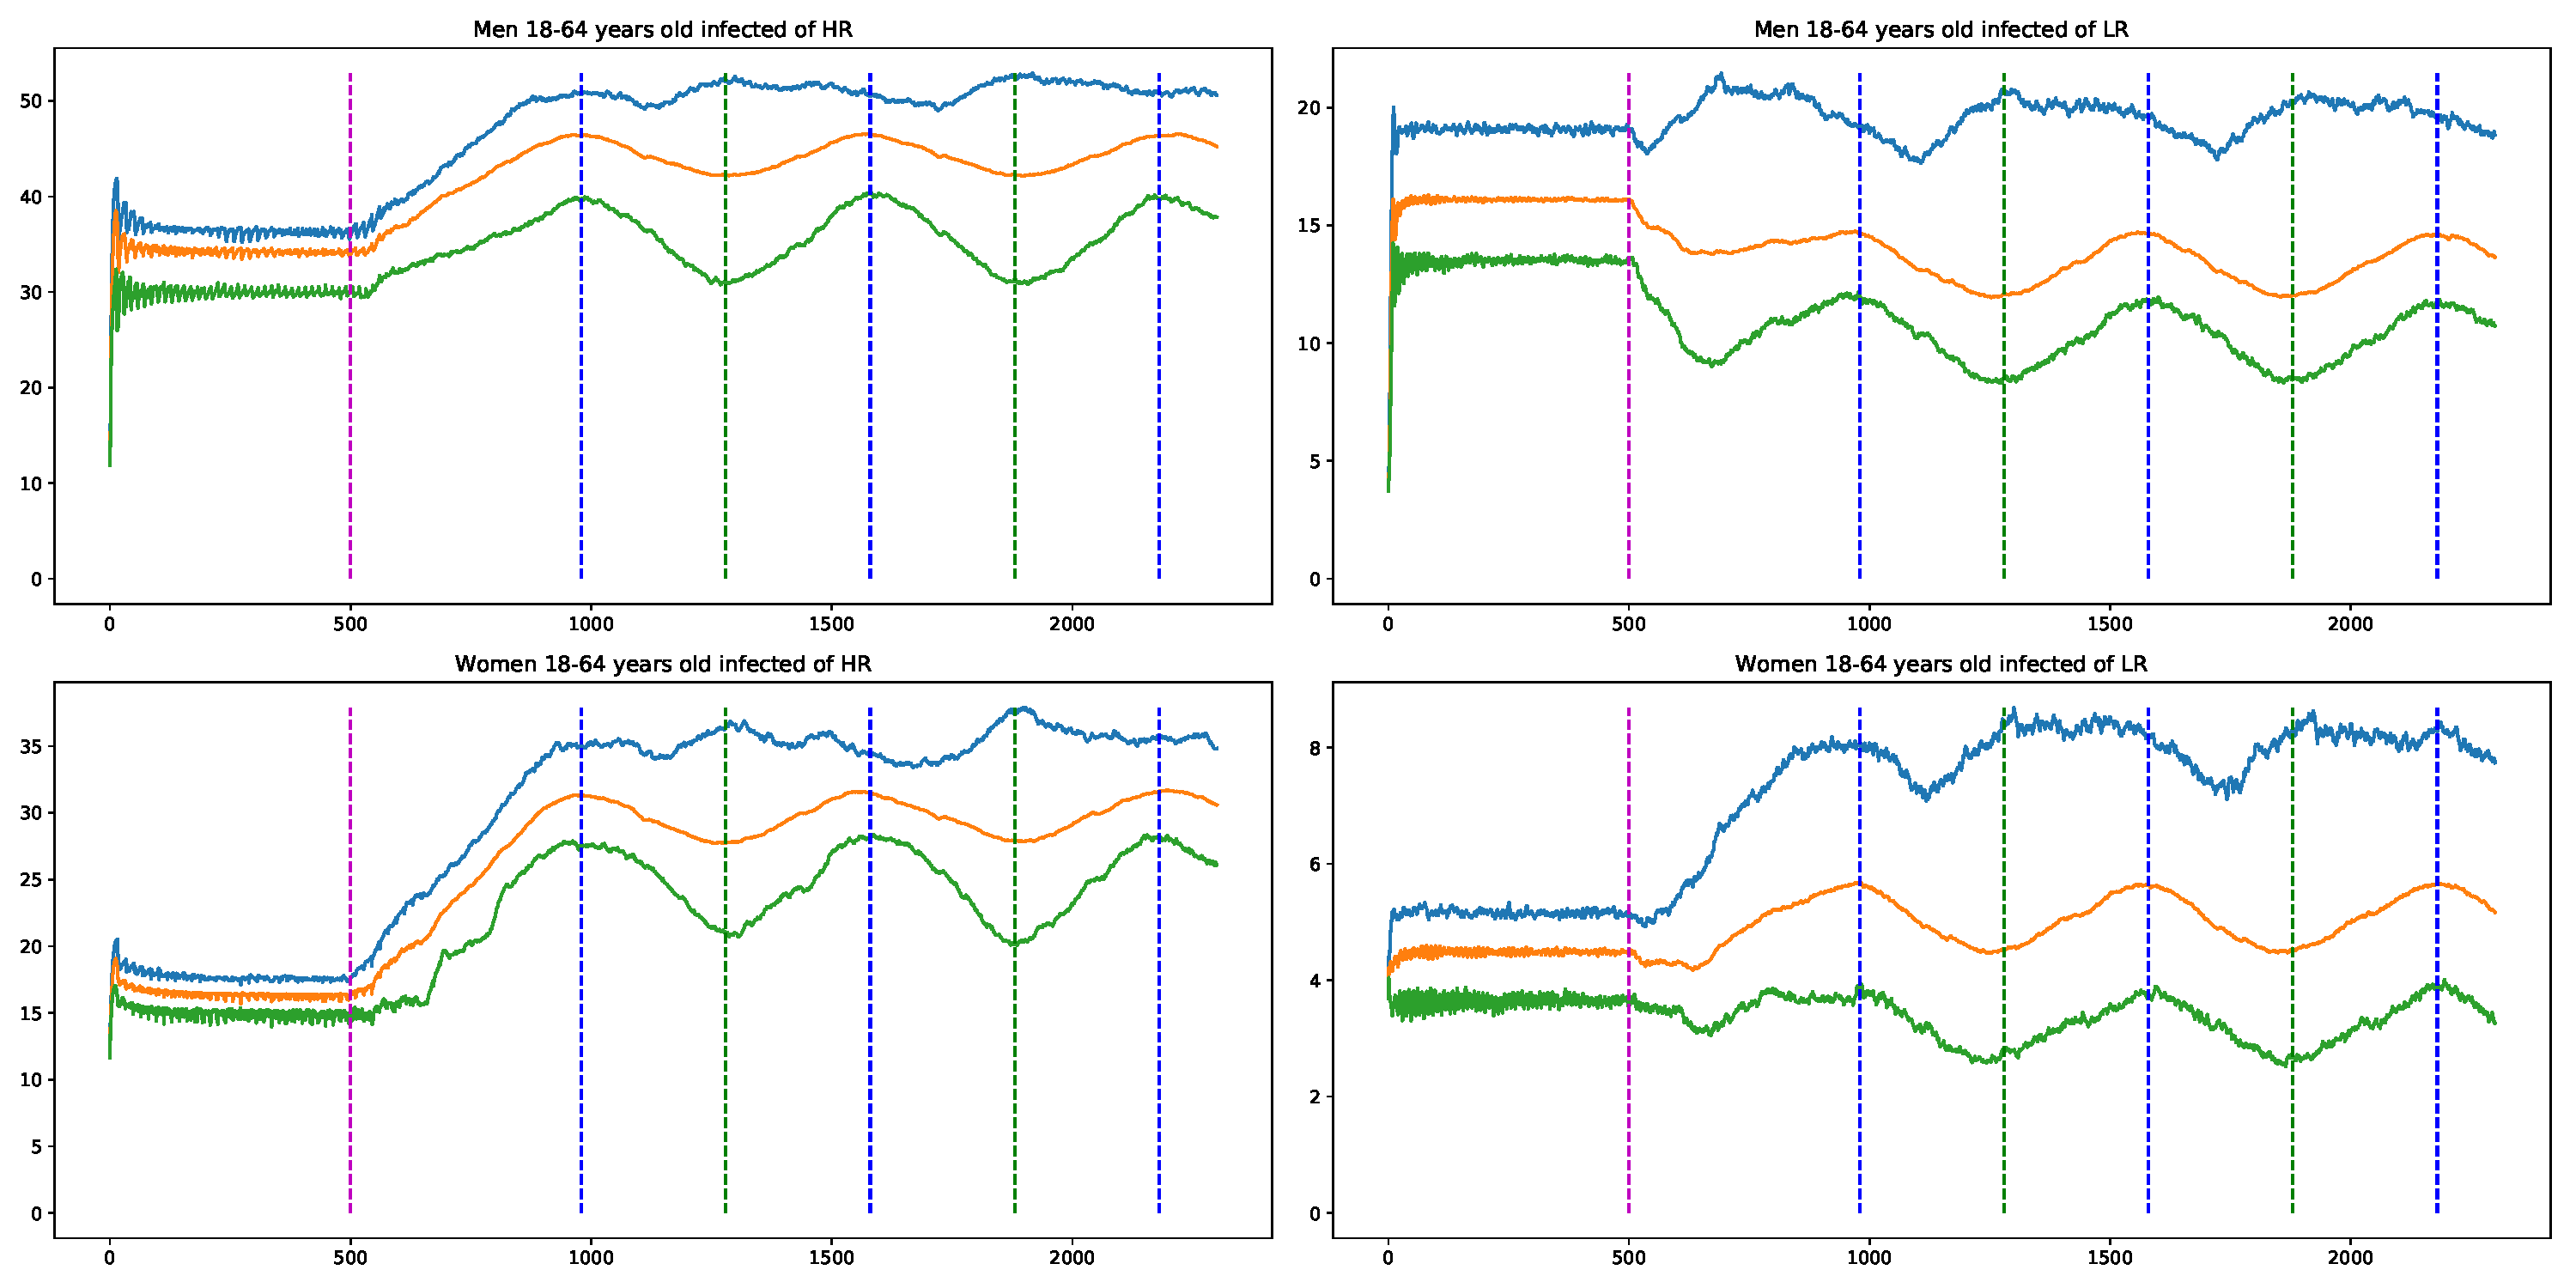
\includegraphics[width=\linewidth]{IMGs/2.-New_features/Estudio_ciclos.pdf}
	\caption{Mean and $95\%$ confidence intervals of the prevalence for 18-64 men and women for HR and LR. Vertical dashed lines indicate milestones of interest. Note the oscillations of the prevalence levels. The blue and green vertical lines correspond to the peaks and valleys of the oscillations. The magenta line, points the month 500 when dynamic network starts.}
	\label{fig:Estudio_ciclos}
\end{figure}

The Figure \ref{fig:Estudio_ciclos} shows the mean and $95\%$ confidence intervals of the $30$ simulations for the prevalence of men and women for HR and LR. The horizontal axis indicates the month and the vertical axis the percentage of infected. As it can be seen, there are oscillation in the evolution of the prevalence.

The vertical lines correspond to:
\begin{itemize}
	\item magenta: month $500$, the static network turns dynamic;
	\item blue: months $980$, $1580$ and $2180$, and point out the peaks in the oscillations in the means and the percentiles. Between them, there are $600$ months ($50$ years), the time of a complete generation in the model;
	\item green: months $1280$  and $1880$, and point out the valleys. Between the valleys there are also $50$ years, and $25$ years between a peak and a valley. 	
\end{itemize}

In some test runs with vaccination, we have observed that, if we start the vaccination schedule when the prevalence is in the decreasing part of the oscillation, the herd immunity appears very much sooner that when we start the vaccination schedule in the increasing part.

If we take into account that in the paper \cite{Ali}, the authors reports extraordinary results in Australia, where two years after the vaccine was introduced, the proportion of genital warts diagnosed declined by a $59\%$ in vaccine eligible young women aged 12--26 years in $2007$, and by $39\%$ in men of the same age, we conjecture that, if there are oscillations in the prevalence of HPV over the time, they have have taken advantage of a decreasing part of the oscillation.

Recall that our goal is to determine the appropriate month where start the vaccination schedule, trying to save computations and favoring the apparition of the herd immunity effect as soon as possible, in order to minimize the opposite effect when the oscillation is in the increasing trend if we have vaccinated a large enough number of individuals.

The oscillations in all the cases, men, women, HR and LR, are very similar, as we can see in the Figure \ref{fig:Estudio_ciclos}, except, maybe in some upper percentiles. Also, there are similarities from the first peak in valleys and peaks. Therefore, in order to take the maximum advantage of the decreasing trends and to save computation, we are going to select the earliest peak, the month $980$, as the starting point for the vaccination.

\subsection{Introducing vaccination} 
For our simulations, we are going to consider the vaccine GARDASIL9 \cite{gardasil9}, that protects against the HPV types 6/11/16/18/31/33/45/52/58. The two first (6/11) are LR and the remainder are HR. Thus, GARDASIL9 protects against $90\%$ of genital wart cases and $90\%$ of the cancer cases \cite{Hartwig2015}. Although GARDASIL9 may protect partially against other HPV types, for modelling purposes we assume that it does not happen. Therefore, it would be interesting to introduce changes in order to monitor if a node is infected by HPV types included in GARDASIL9 or not, and then, to simulate accurately the protection effect of the vaccine.

Following the study conducted in \cite{castellsague2012prevalence}, if a woman is infected by HPV LR, the probability to be only infected by 6/11 is $34.23\%$, $63.06\%$ only infected by others than 6/11 and $2.70\%$ to be infected by both. Also, if a woman is infected by HPV HR, the probability to be infected only by 16/18/31/33/45/52/58 is $30.44\%$, $23.66\%$ only infected by others than 16/18/31/33/45/52/58 and $45.90\%$ by both. Due to the lack of information about men, we will also use the above percentages for men.

Then, before starting the vaccination, we label men and women as infected of HPV LR 6/11 or infected of HPV LR other than 6/11 or infected of both, following the above percentages. Analogously, we label men and women as infected of HPV HR 16/18/31/33/45/52/58 or infected of HPV HR other than 16/18/31/33/45/52/58 or infected of both.

Once these assignments are done, we continue with the HPV transmission dynamics including the vaccination, taking into account the new labels we included. If a node has been vaccinated, it can be infected by the types of HPV different to those that GARSDASIL9 protects and, in this case, they will never be infected of 6/11 nor 16/18/31/33/45/52/58. If a node has not been vaccinated, can be infected by any HPV type. 

The assumed effectiveness of the vaccine is $96.5\%$.

\subsection{Introducing vaccination loss protection}
In the previous section we assume that the protection of GARDASIL9 is forever. In fact, until now, people vaccinated by GARDASIL (previous version of GADASIL9) do not have experienced any loss in the protection. But this does not mean that it could happen in the future. 

In fact, we want to simulate the worst possible scenario, that is, the sudden drop to zero of the protection. To simulate this possibility, we will introduce a new parameter that represents the time after the vaccination where the protection is complete. Therefore, after this time, the vaccinated individual will behave as a non-vaccinated individual.

\subsection{Introducing variations in the vaccination coverage}
One of our goals is to simulate scenarios where variations in the vaccination coverage have been occurred and we want to study the effect in the global protection against HPV due to these variation of the coverage. To simulate these scenarios, we will include into the model vectors of coverage, indicating the vaccine coverage every month, and vaccinating the people following these variable coverages. 

%Cap�tulo 5 - caso AUS de revista Viruses
%Aqui hay que mezclar sabiamente y en orden el paper de Viruses y los resultados del informe
\chapter{Australian case}\label{Australiano}

In this chapter we are going to check if we can obtain similar results to those in \cite{ali2013genital,fairley2009rapid} using the parameters of the new calibration.

As we introduced in Chapter \ref{intro} there is a decrease on the number of infected persons and the number of persons with GW is already reported for Australia after two years of administering vaccinations to young girls. These results were more impressive than predicted by continuous models.

To check the reliability of the model, we simulated the HPV vaccination campaign carried out in Australia \cite{ali2013genital}, and compared them with the actual impact published \cite{ali2013genital}. In 2007, Australian health authorities started a vaccination program for 12--13 year-old girls with a~coverage of $73\%$ ($83\%$ in the first dose, $80\%$ in the second dose and $73\%$ in the third dose). In addition, from 2007 to 2009, there was a catch-up vaccination program for women aged 13--26 with a decreasing coverage with age until $52\%$ in women aged 20--26. Their results can be summarized as follows \cite{ali2013genital}:

\begin{itemize}
	\item Two years after the vaccine was introduced, the proportion of genital warts diagnosed declined by a $59\%$ in vaccine eligible young women aged 12--26 years in $2007$, and by $39\%$ in men of the same age.
	\item No significant decline was observed in women or men older than $26$ years old, non-resident young women, or men who have sex with men.
\end{itemize}

Two different scenarios were considered to be simulated:

\begin{itemize}
	\item Scenario 1: vaccination of $83\%$ of the $14$ year-old girls (or younger girls) plus a catch-up with coverage $73\%$ for 14--26 year-old women.
	\item Scenario 2: vaccination of $73\%$ of $14$ year-old girls (or younger girls) plus a catch-up with a~vaccination coverage of $52\%$ for 14--26 year-old women.
\end{itemize}

These simulations represented the upper and lower bounds of the scenario implemented in Australia. 

\section{How to measure the decline}\label{sec:decline}%esto lo borré de otro capítulo y lo pongo ya aqui

We call $I$ the number of infected women of LR HPV 6 and/or 11 just before the starting of the vaccination campaign; we call $V = ( v_1, \ldots, v_N)$ to the number of infected women of LR HPV 6 and/or 11 every month from the starting of the vaccination program until the end of the simulation. Then,~the~vector 

\begin{equation}
100 \times \left( 1-\displaystyle\frac{v_1}{I}, \ldots, 1-\displaystyle\frac{v_N}{I} \right) \; 
\end{equation}
is a measure of the percentage of decline of number of infected women of LR HPV 6 and/or 11 after the beginning of the vaccination campaign. This will also be applied to men and MSM.

In order to compare GW data given in \cite{ali2013genital} with our model, results referred to infected women of LR HPV 6 and/or 11, we should take into account that, whether a fixed proportion of HPV 6 and/or 11 infected individuals develops warts, the percentage of decline in warts and in infected women of LR HPV 6 and/or 11 will be comparable. 

Another important issue for the natural history of the disease is the persistence of the infection \cite{campos2014updated}. Our model does not consider the persistence ``a priori'', but we derive the cases of genital warts from the number of cases of infected individuals by taking this data into account.



\section{Does our model return similar values to those in \cite{ali2013genital}?}
In this section, we are going to show figures about prevalence or decline of the percentage of women, men and MSM infected of LR 6/11, the HPV type responsible of $90\%$ of genital warts. Taking into account that genital warts, in average, use to appear 6 months after the infection, the figures about prevalence or decline will be a good estimation of the prevalence and the  decline of genital warts.  

Figure \ref{fig:prev_AUS_6_11} shows the percentage of women, men and MSM aged 14-26 infected of LR 6/11 after starting the vaccination program in both simulated scenarios. We can see the fast decrease for women and men in both scenarios from the very beginning. MSM, remain constant. 

\begin{figure}[!]
	\centering
	\begin{tabular}{cc}
		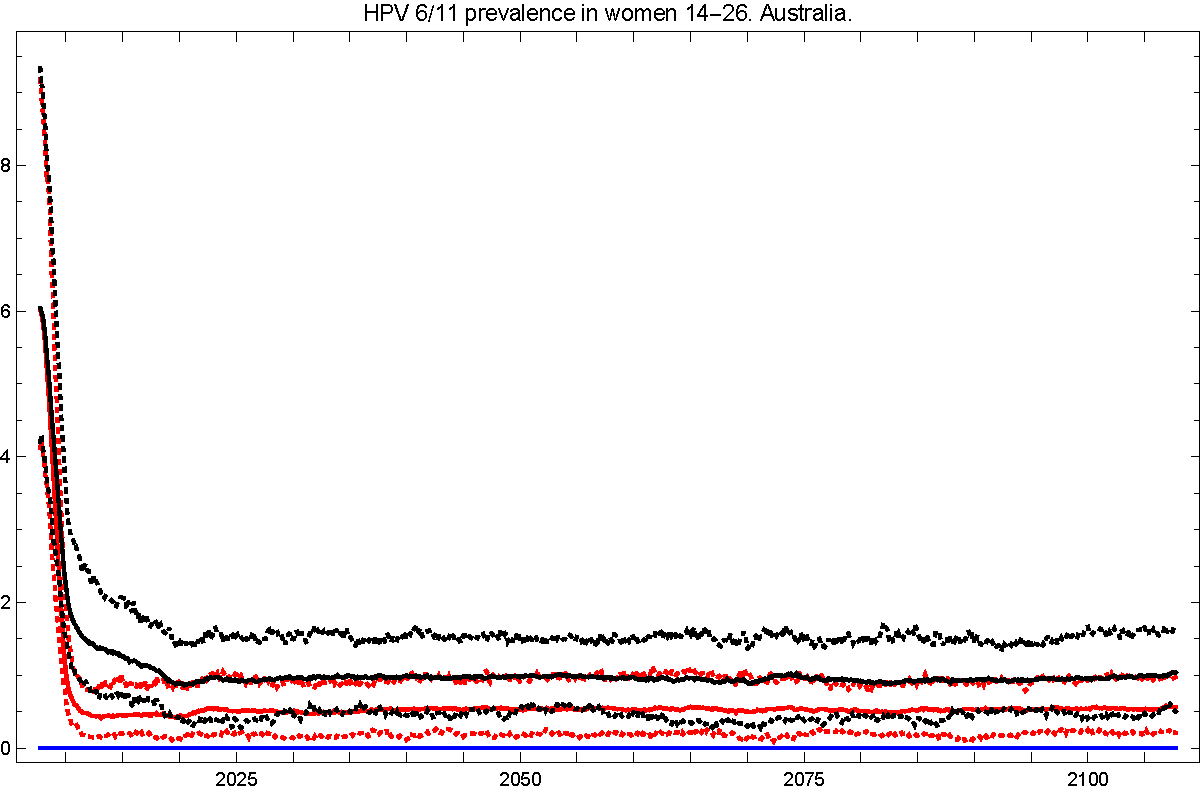
\includegraphics[width=0.5\linewidth]{IMGs/3.-Australia/Retr_muj_14_26_verr_Australia.pdf}	& 
		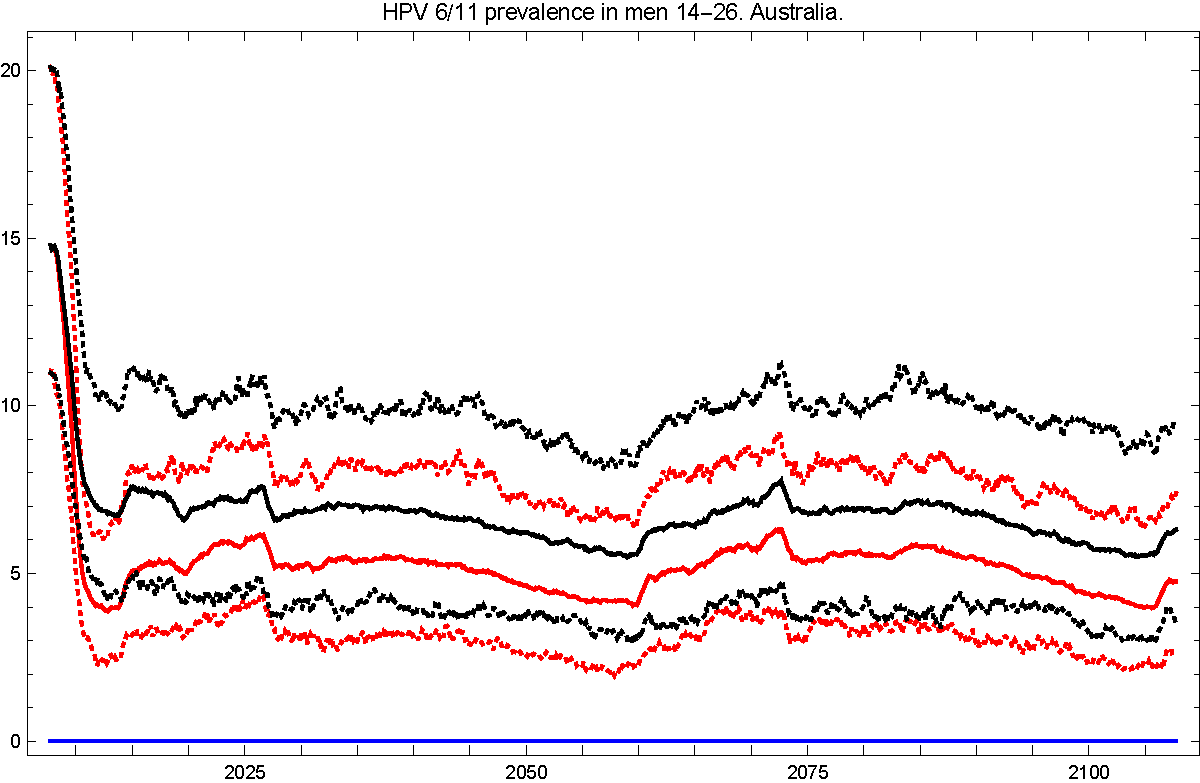
\includegraphics[width=0.5\linewidth]{IMGs/3.-Australia/Retr_hom_14_26_verr_Australia.pdf}  \\ 
		(a)	& (b) \\ 
		\multicolumn{2}{c}{ 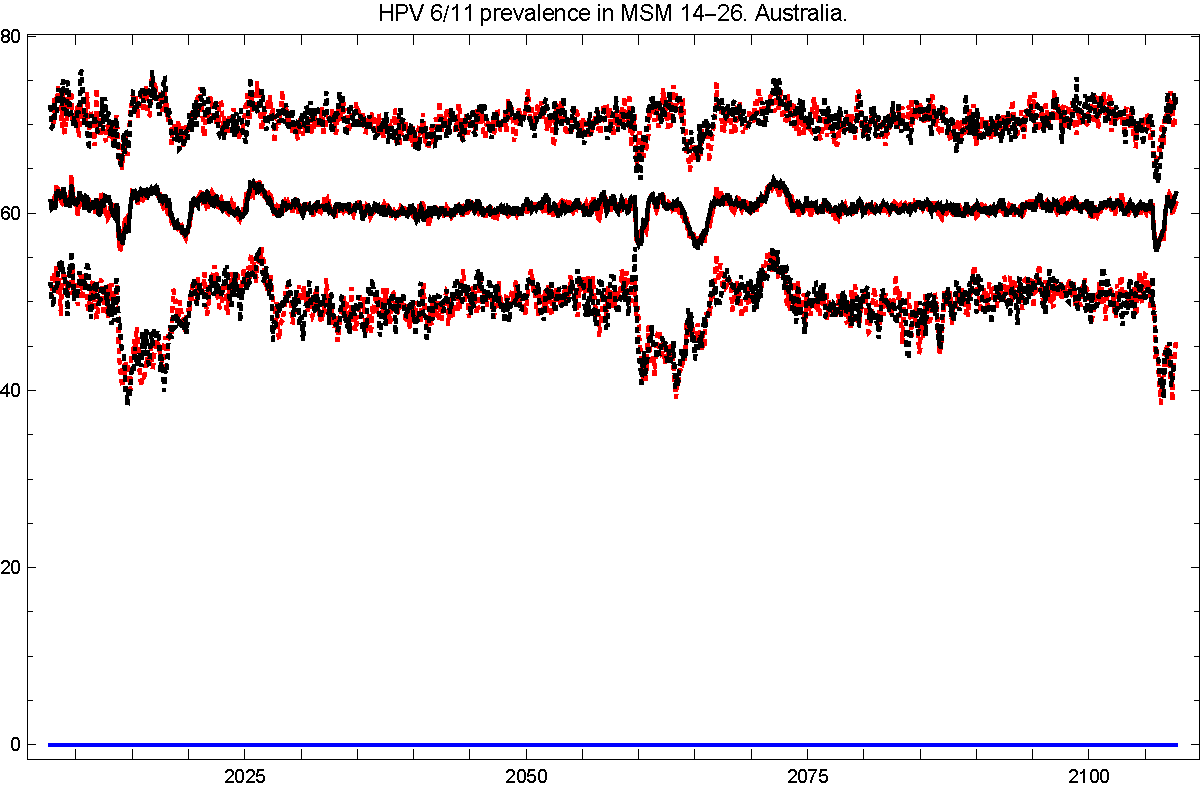
\includegraphics[width=0.5\linewidth]{IMGs/3.-Australia/Retr_MSM_14_26_verr_Australia.pdf} } \\ 
		\multicolumn{2}{c}{(c)} \\ 
	\end{tabular} 
	\caption{Percentage of women (a), men (b) and MSM (c) aged 14-26 infected of LR HPV 6 and/or 11 after the implementation of the vaccination program. The red lines correspond to the average and $95\%$ confidence interval for Scenario 1 and the black lines to Scenario 2.  We can see the fast decrease for women and men in both scenarios from the very beginning. However, there is not effect on MSM.}
	\label{fig:prev_AUS_6_11}	
\end{figure}

In Figure \ref{fig:decline_AUS_6_11}, we have plotted the same data as in Figure \ref{fig:prev_AUS_6_11} but from another point of view: the average percentage of decline of women and men infected of LR HPV 6 and/or 11. As the vaccination program progresses over time, the percentage of decline obviously grows. After 2 years, the model shows a decline of

\begin{itemize}
	\item Scenario 1: $72.0\%$ with CI $95\%$ $[67.7\%, 76.5\%]$ for women and $38.9\%$ with CI $95\%$ $[32.0\%, 45.5\%]$ for men. 
	\item Scenario 2: $54.8\%$ with CI $95\%$ $[48.5\%, 59.0\%]$ for women and $27.7\%$ with CI $95\%$ $[21.3\%, 34.5\%]$ for men. 
\end{itemize}

Australian reported levels of decline ($59\%$ in women and $39\%$ in men aged 14-26) will be reached by the model after

\begin{itemize}
	\item Scenario 1: $1.66$ years with CI $95\%$ $[1.5, 1.75]$ for women and $2.0$ years with CI $95\%$ $[1.75, 2.16]$ for men,
	\item Scenario 2: $2.1$ years with CI $95\%$ $[2.0, 2.33]$ for women and $2.42$ years with CI $95\%$ $[2.08, 2.83]$ for men.
\end{itemize}

\begin{figure}[!]
	\centering
	\begin{tabular}{cc}
		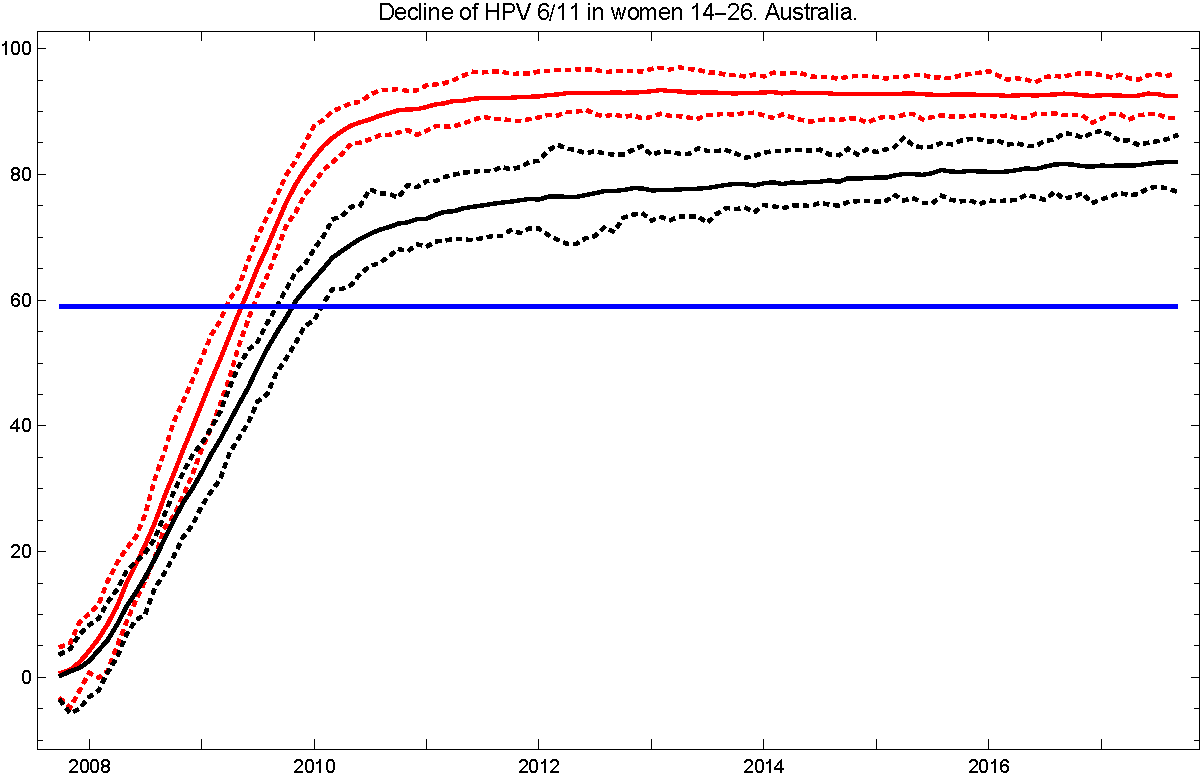
\includegraphics[width=0.5\linewidth]{IMGs/3.-Australia/Decl_muj_14_26_verr_Australia.pdf}	& 
		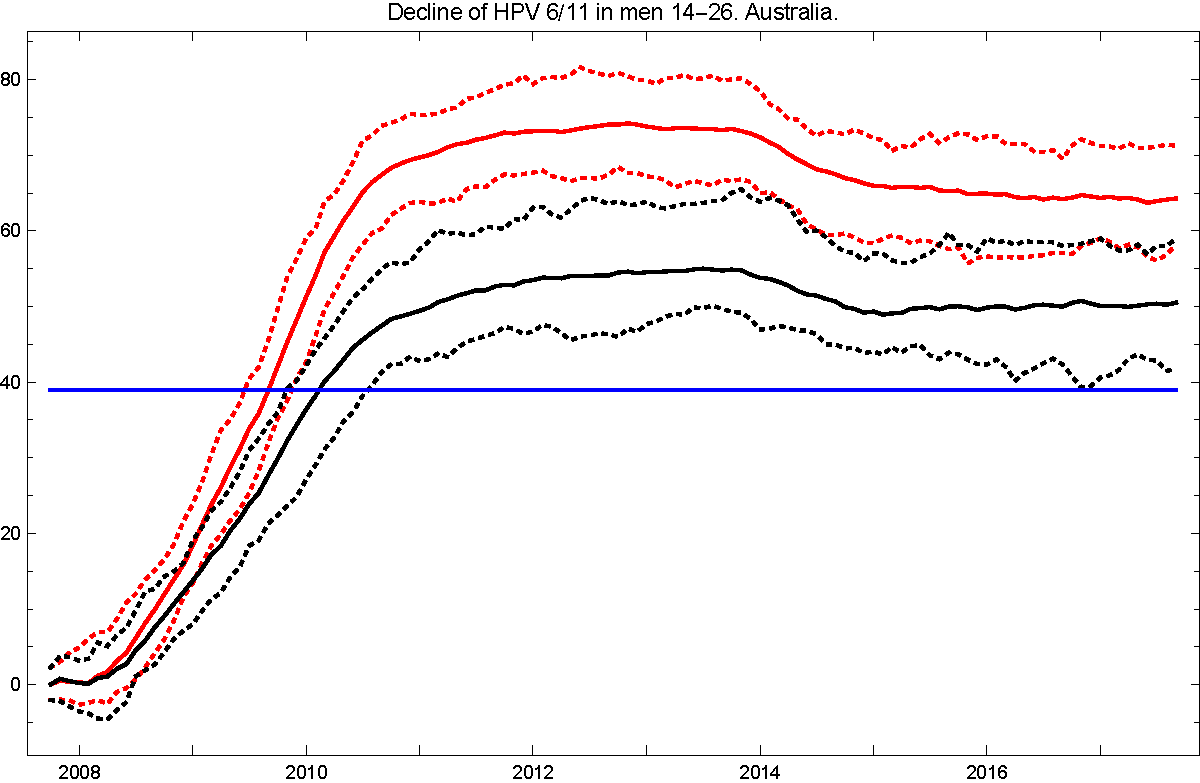
\includegraphics[width=0.5\linewidth]{IMGs/3.-Australia/Decl_hom_14_26_verr_Australia.pdf}  \\ 
		(a)	& (b) 
	\end{tabular} 
	\caption{Percentage of decline of women (a) and men (b) aged 14-26 infected of LR HPV 6 and/or 11 (and consequently of genital warts) after the implementation of the vaccination program. The red lines correspond to the average and $95\%$ confidence interval for Scenario 1 and the black lines to Scenario 2. After 2 years, the model shows a decline of $72\%$ for Scenario 1 and $54.8\%$ for Scenario 2, in average, for women and $38.9\%$ for Scenario 1 and $27.7\%$ for Scenario 2, in average, for men.}
	\label{fig:decline_AUS_6_11}
\end{figure}

No significant impact on the rate of infection was observed in men aged 27-64 and women 2 years after the implementation of the vaccination program (Figure \ref{fig:decline_AUS_6_11_27_64}) and the same in women agreeing the observations reported in \cite{ali2013genital}. It can be explained by the fact that, usually, individuals have sexual intercourses with people more or less the same age.

Then, our model predict figures close to the ones given in \cite{ali2013genital}.

\begin{figure}[!]
	\centering
	\begin{tabular}{cc}
		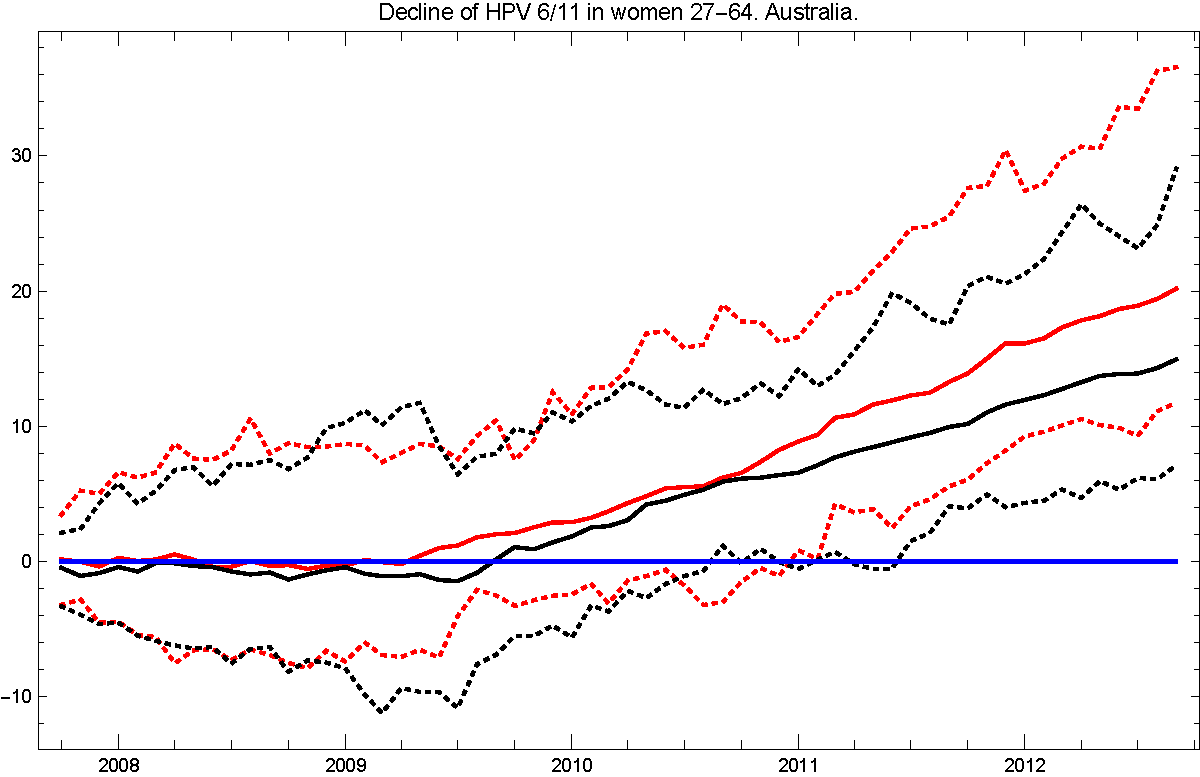
\includegraphics[width=0.5\linewidth]{IMGs/3.-Australia/Decl_muj_27_64_verr_Australia.pdf}	& 
		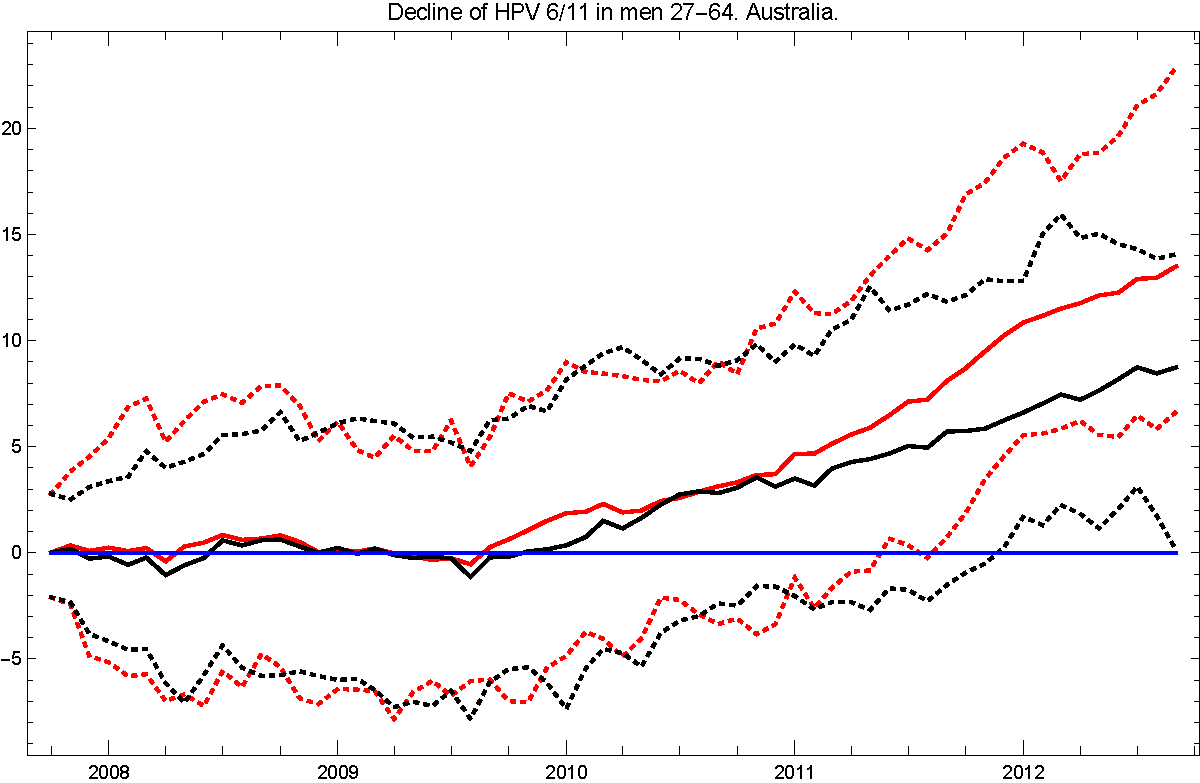
\includegraphics[width=0.5\linewidth]{IMGs/3.-Australia/Decl_hom_27_64_verr_Australia.pdf}  \\ 
		(a)	& (b) 
	\end{tabular} 
	\caption{Percentage of decline of women (a) and men (b) aged 27-64 infected of LR HPV 6 and/or 11 (and consequently of genital warts) after the implementation of the vaccination program in both scenarios. The red lines correspond to the average and $95\%$ confidence interval for Scenario 1 and the black lines to Scenario 2. Notice that, in average, no significant decline appears in the 5 years after the implementation of the vaccination program.}
	\label{fig:decline_AUS_6_11_27_64}
\end{figure}

\section{Study of the herd immunity effect over HPV LR infection}
The herd immunity effect in both scenarios is shown in Figure \ref{fig:decline_AUS_6_11_14_64} for women, men and MSM. Notice that, in men and MSM, any decline is due to herd immunity. The decline in the whole female population appears when the lines representing their decline are over the vaccination lines (green for Scenario 1 and orange for Scenario2) also shown in this figure. We see that the herd immunity effect starts after 

\begin{itemize}
	\item for women
	\begin{itemize}
		\item Scenario 1: $0.58$ years with CI95\% $[0.0, 22.1]$.
		\item Scenario 2: $0.58$ years with CI95\% $[0.0, 22.1]$.
	\end{itemize}
	\item for men
	\begin{itemize}
		\item Scenario 1: $0.0$ years with CI95\% $[0.0,0.83]$.
		\item Scenario 2: $0.0$ years with CI95\% $[0.0,0.83]$.	
	\end{itemize}
\end{itemize}

The herd immunity effect starts very quickly for men. For MSM, there is not a clear herd immunity effect because the decline is stable over the time. For women, we can see that, practically, the CI$95\%$ decline lines are over the vaccination lines in both scenarios. This means that, in the worst case, only the vaccinated women will be protected and in the best case, almost all women will be protected by vaccination or by herd immunity effect.

\begin{figure}[!]
	\centering
	\begin{tabular}{cc}
		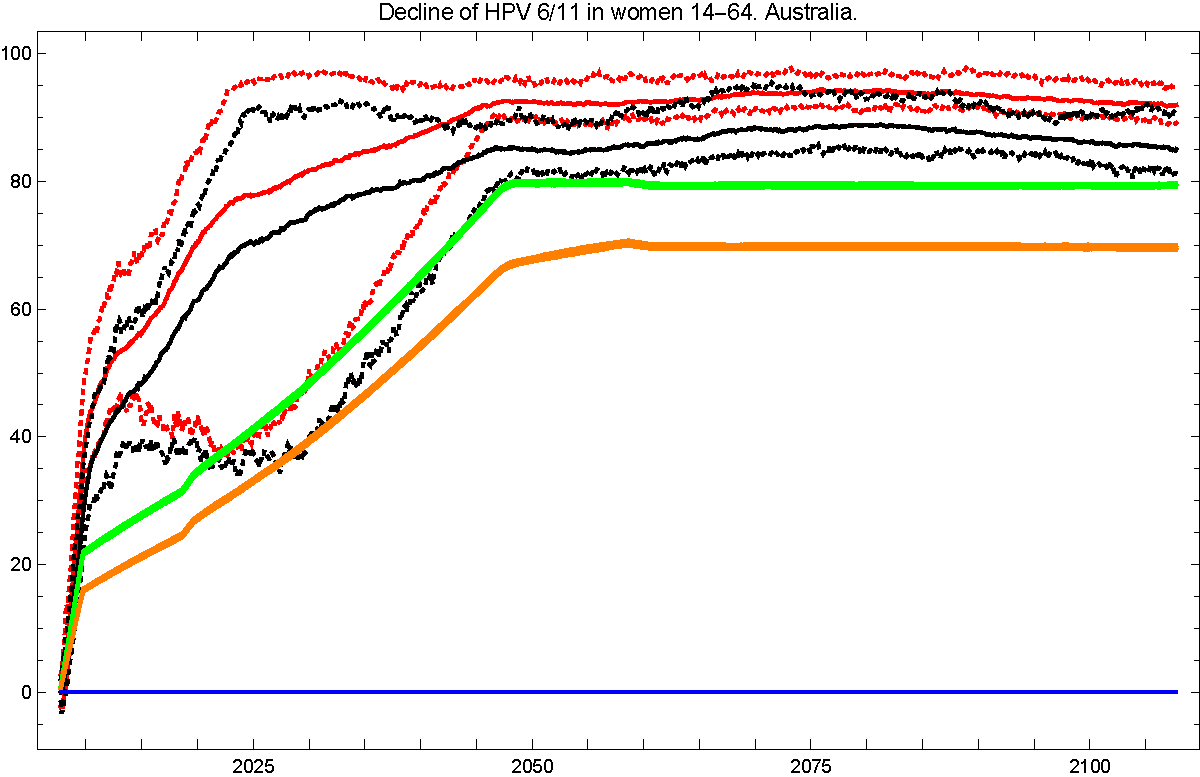
\includegraphics[width=0.5\linewidth]{IMGs/3.-Australia/Decl_muj_14_64_verr_Australia.pdf}	& 
		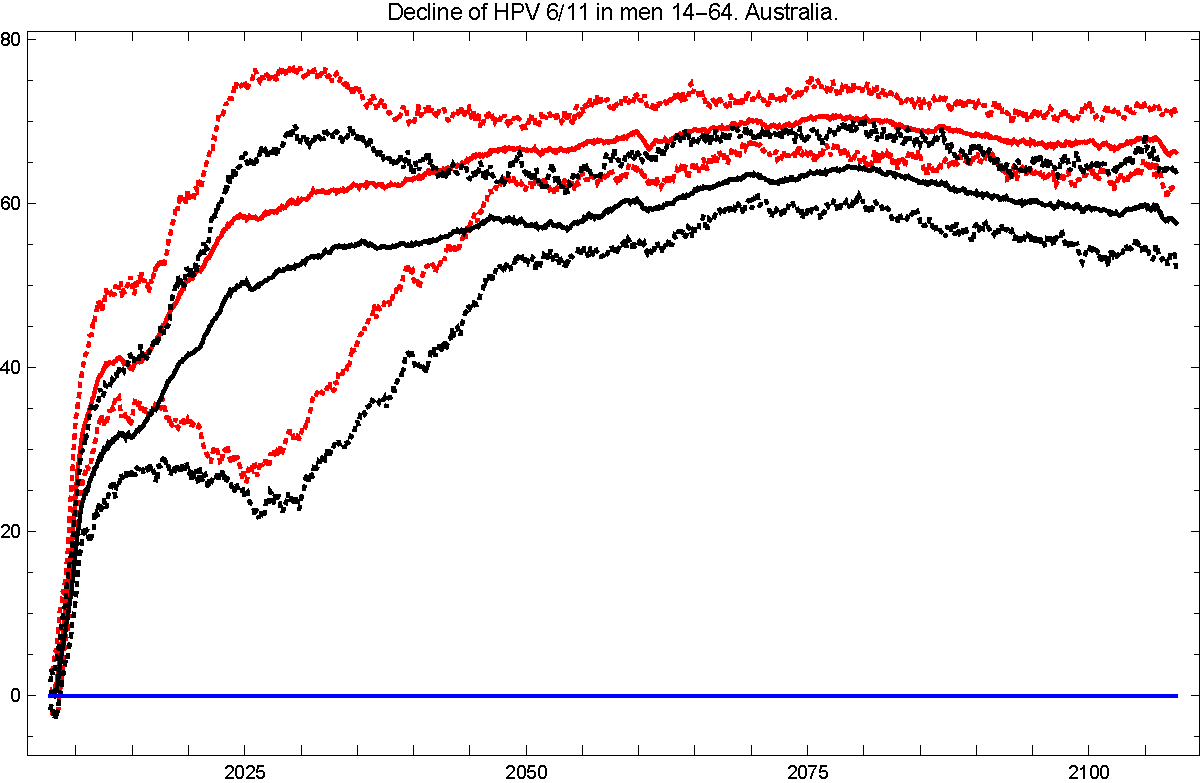
\includegraphics[width=0.5\linewidth]{IMGs/3.-Australia/Decl_hom_14_64_verr_Australia.pdf}  \\ 
		(a)	& (b) \\ 
		\multicolumn{2}{c}{ 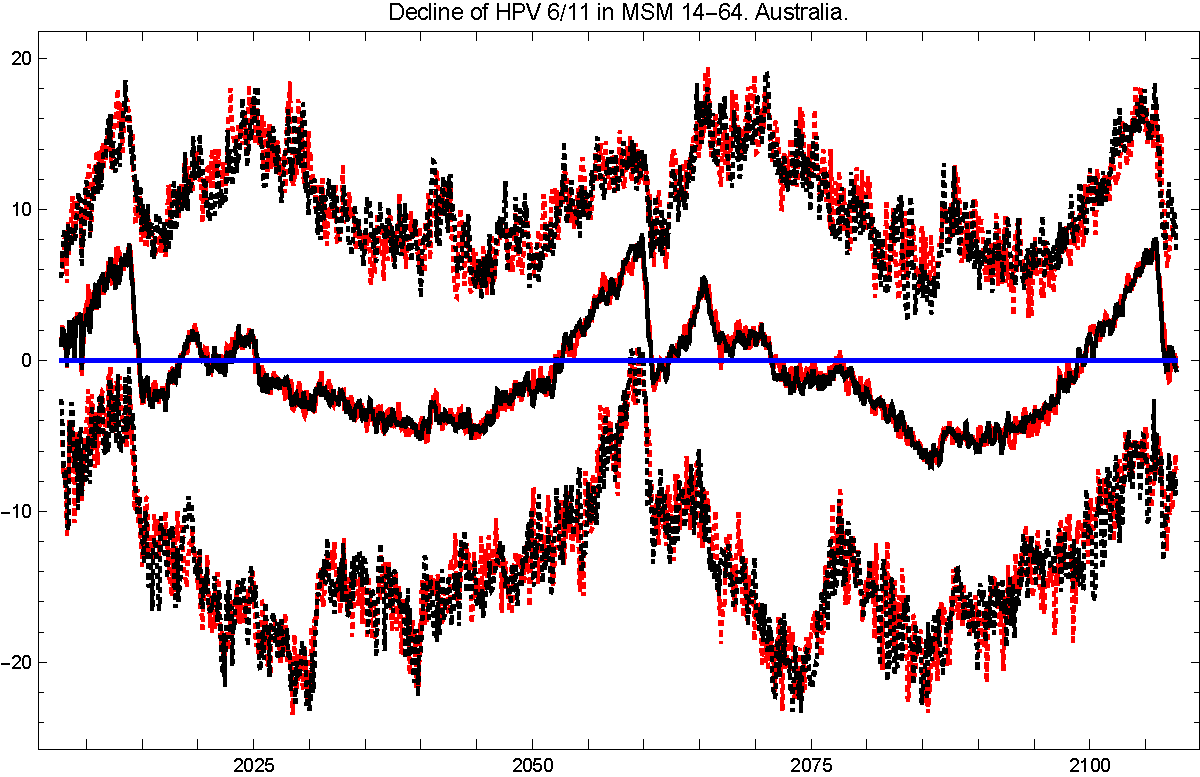
\includegraphics[width=0.5\linewidth]{IMGs/3.-Australia/Decl_MSM_14_64_verr_Australia.pdf} } \\ 
		\multicolumn{2}{c}{(c)} \\ 
	\end{tabular} 
	\caption{Percentage of decline of women (a), men (b) and MSM (c) aged 14-64 for the vaccination program in Australia. The red lines correspond to the average and $95\%$ confidence interval for Scenario 1 and the black lines to Scenario 2. In the figure (a), green and orange lines correspond to women vaccination percentage for Scenario 1 and 2, respectively. Notice that the herd immunity effect contributes to the decline in the number of infections in men and the decline in the number of infections for unvaccinated women. This latter can be seen when the decline lines are over the vaccination line. However, any herd immunity effect can be seen in MSM.}
	\label{fig:decline_AUS_6_11_14_64}
\end{figure}

Notice that the herd immunity effect is very clear within the CI$95\%$ both for women and men, but it does not appear in the MSM population. In the best case scenario, the MSM subpopulation achieves a constant protection level of $10\%-15\%$. This could be attributed to the way in which the MSM individuals are connected: with a very large number of LSPs among them and some casual links with women with large LSPs.

\section{Discussion}
The random network of sexually transmitted HPV including up to $100,000$ nodes, was developed to fit the data of surveys concerning the number of sexual partners throughout life. Standard continuous models are insufficient to accurately predict transmission because they do not account for the individual to individual transmission of the infection, the role of hubs in disseminating the virus through the rest of the population and neither the vaccination campaigns targeting specific groups of individuals.

This network has successfully been applied to the stable state of infections by LR and HR HPV genotypes in Spain  \cite{Acedo2017}. In this study we mimicked the results found in the HPV vaccination campaign in Australia \cite{ali2013genital}, and showed very reliable results. 

Models based upon continuous differential equations predict a slower decrease in the number of infected individuals after implementing similar vaccination campaigns \cite{elbasha2007model}. Hence, the case of the HPV vaccination in Australia provides one of the best real scenarios for testing new network models in mathematical epidemiology. There is an on-going debate on the pertinence of an approach based upon networks on epidemiology \cite{Eubank} and this work contributes to show the necessity of such an approach in many cases, in particular, in those corresponding to STD.

To validate the model, we used the Australian experience, with two different vaccination coverages: routinely vaccination campaign for $12-13$ year-old girls with a coverage of $73\%$ and $83\%$ and a catch-up program in the $14-26$ age group with an average coverage of $52\%$ and $73\%$. This program revealed an important herd effect \cite{ali2013genital}, so that vaccination decreased the incidence of genital warts (GW) even in the non-vaccinated men because of the protection of infection conferred by the vaccine, and the decreased transmission of the virus.

The model predicted a fast decline in the number of infections parallel to the decline in the number of GW in Australia with very similar values. However, this model was built with Spanish data on sexual behavior \cite{INE} and prevalence of HPV infection \cite{castellsague2012prevalence}, that might differ to the Australian one, and may explain the minor differences found between the model and the actual data published. Herd immunity in this model of STD is predicted much sooner than in other highly transmitted aerial transported infectious diseases as influenza or RSV, due to the structure of the network. This supports the need to build appropriate LSP networks. 

Other models have also predicted the protection of males by vaccinating girls and women, but only for men, as the model used by Bogaards et al. \cite{bogaards2015direct}. This model uses Bayesian techniques to study the herd immunity effect. However, in contrast with our model, it does not take into account the dynamics of the HPV transmission, the importance of age-groups and the different roles they play in the propagation of these viruses or the links among the MSM subpopulation and the heterosexual network. In this sense, a network model is required to study the impact of the vaccination strategies in short, medium and long time scales.

Vaccination strategies should seek an optimal effectiveness and efficiency. In this case, it can be seen the quick apparition of the herd immunity effect on males and females only vaccinating women. However, the herd immunity effect does not appear in  MSM. This can be the consequence of the large LSP numbers for MSM and their casual connections with women with large LSP numbers in the heterosexual subnetwork.

The model considers a quiet close community, where there is not much contact with other communities. This may not be the case in Spain which in $2016$ received over $75$ million tourists \cite{INEturismo}, representing almost the double of the number of Spanish inhabitants, and when sexual contacts are frequent. This may bias the results, as the herd immunity in Spain may not be so clear as in countries with less tourism. Nevertheless we will study the effect of tourism in Spain.

Another issue that we must take into account, is the modelling of the population with a high number of contacts because these individuals are hubs in the network whose vaccination may induce a faster decline of the virus prevalence. Our approach is rather conservative in the assignment of LSP for men and women with $10$ or more links because we assume that all of them have similar LSP. However, it is expected that individuals with extreme values of LSP are favouring the transmission of HPV in such a way that  a targeted vaccination can show its benefit in a very short time.


\begin{thebibliography}{99}


\bibitem{Pathology}
Sirj\"anen, K.; Sirj\"anen, S. Papillomavirus Infections in Human Pathology. Wiley \& Sons: New York,~2000.

%2
\bibitem{Roberts} Roberts, J.S.C. Vaccine for Genital Warts. In {\em Vaccines for Human Papillomavirus Infections and Anogenital Disease}; Tindle, R.W., Ed.; Medical Intellegence Unit 14, R. G. Landes Company: Austin, TX, USA, 1999.

%3
\bibitem{CLEOPATRE} Castellsagu\'e, X.; Iftner, T.; Roura, E.; Antonio Vidart, J.; Kjaer, S.K.; Bosch, F.X.; Mu�oz, N.; Palacios,~S.; San Martin Rodriguez, M.; Serradell, L.; et al.  Prevalence
and genotype distribution of human papillomavirus infection
of the cervix in Spain: the CLEOPATRE study. {\em J. Med. Virol.} {\bf 2012}, {\em 84}, 947--956, doi:10.1002/jmv.23282.

%4
\bibitem{McNeil} McNeil, C. Who invented the VLP Cervical Cancer Vaccines? {\em J. Natl. Cancer Inst.}
{\bf 2006}, {\em 98}, 433.

%5 
\bibitem{Elbasha1} Elbasha E.H.; Dasbach E.J.; Insinga R.P. Model for assessing human papillomavirus vaccination strategies. {\em Emerg. Infect. Dis.} {\bf 2007}, {\em 13}, 28--41.

%6
\bibitem{Elbasha2} Elbasha, E.H.; Galvani, A.P. Vaccination against multiple HPV types. {\em Math. Biosci.} {\bf 2005}, {\em  197}, 88--117.

%7
\bibitem{Fairley} Fairley, G.; Hocking, J.; Chen, M.; Donovan, B.C. Rapid decline in warts after national quadrivalent HPV vaccine program. In Proceedings of the 25th International Papillomavirus Conference, Malmo, Sweden, 8--14~May 2009. 

%8
\bibitem{Ali} Ali, H.; Donovan, B.; Wand, H.; Read, T.R.H.; Regan, D.G.; Grulich, A.E.;
Fairley, C.K.;  Guy, R.J. Genital~warts in young australians five
years into national human papillomavirus vaccination programme: National surveillance
data. {\em BMJ} {\bf 2013}, {\em 346}, f2032.

%9
\bibitem{Bogaards} Bogaards, J.A.; Wallinga, J.; Brakenhoff, R.H.; Meijer Chris, J.L.M.; Berkhof, J. Direct benefit of vaccinating boys along with girls against oncogenic human papillomavirus: Bayesian evidence synthesis. \textit{BMJ} \textbf{2015}, \textit{350}, h2016. 

%10
\bibitem{RSV} Acedo, L.;  Mora\~no, J.A.; Villanueva, R.J.; Villanueva-Oller, J.; D\'{\i}ez-Domingo, J. Using random networks to study the dynamics of respiratory syncytial virus (RSV) in the Spanish region of Valencia. {\em Math. Comp. Mod.} {\bf 2011},
{\em 54}, 1650--1654.

%11
\bibitem{Obesity} Christakis, N.A.; Fowler, J.H. The Spread of Obesity in a Large Social Network over 32 Years. {\em N. Engl. J.
	Med.} {\bf 2007}, {\em 357}, 370--379.

%12
\bibitem{HPV}  Burchell, A.;  Richardson, H.;  Mahmud, S.M.; Trottier, H.; Tellier, P.P.;  Hanley, J.;  Coutl\'ee, F.;  Franco,~E.L. Modeling the Sexual Transmissibility of Human Papillomavirus Infection using Stochastic Computer Simulation and Empirical Data from a Cohort Study of Young Women in Montreal, Canada. {\em  Am.~J.~Epidemol.} {\bf 2006}, {\em 169}, 534--543.

%13
\bibitem{Web} Liljeros, F.; Edling, C.R.; Nunes, L.A.; Stanley, H.E.;  \r{A}berg, Y. The web of human sexual contacts. {\em Nature} {\bf 2001}, {\em 411}, 907--908.

%14
\bibitem{Bearman} Bearman, P.S.;  Moody, J.; Stovel, K. Chains of Affection: The Structure of
Adolescent Romantic and Sexual Networks. {\em Am. J. Sociol.} {\bf July 2004}, {\em 110}, 44--91.

%15
\bibitem{Likoma} Helleringer, S.; Kohler, H.P. Sexual network structure and the spread of HIV in
Africa: evidence from Likoma Island, Malawi. {\em AIDS} {\bf 2007}, {\em 21}, 2323--2332.

%16
\bibitem{Schmid} Schmid, B.V.; Kretzschmar, M. Determinants of sexual network structure and their impact on cumulative
network measures. {\em PLoS Comput. Biol.} {\bf 2012}, {\em 8}, e1002470.

%17
\bibitem{IVE} Portal estadistico de la Generalitat Valenciana (Statistical Portal of the Government of the Community of Valencia) (2013). Available online: \url{http://www.ive.es} (accessed on 6 March 2017)

%18
\bibitem{INE} Encuesta de Salud y H\'abitos Sexuales 2003. (Health and Sexual Habits Survey 2003). July 2004. Instituto Nacional de Estad\'{\i}stica. Available online:\url{http://www.ine.es} (accessed on 6 March 2017)
%http://www.ine.es/dyngs/INEbase/es/operacion.htm?c=Estadistica_C&cid=1254736176785&menu=resultados&idp=1254735573175

%19
\bibitem{Acedo2013} Acedo, L. Mora\~no, J.-A., Brain oscillations in a random neural network. {\em Math. Comput. Model.}
{\bf April 2013}, {\em 57}, 1768--1772. \url{https://doi.org/10.1016/j.mcm.2011.11.028}

%20
\bibitem{Dorogovtsev} Dorogovtsev, S.N.; Mendes, J.F.F. \emph{Evolution of Networks: From Biological Networks to the Internet and WWW};
Oxford University Press; Reprint edition  Oxford, UK (January 14, 2014).

%21
\bibitem{Watts} Watts, D.J.; Strogatz, S.H. Collective dynamics of small-world networks. \emph{Nature} {\bf 1998}, {\em 393}, 440--442.

%22
\bibitem{USA2} Key Statistics from the National Survey of Family Growth. Available online: \url{http://www.cdc.gov/nchs/nsfg/key\_statistics/n.htm} (accessed on 14 October 2017).

%23
\bibitem{USA} Chandra, A.; Mosher, W.D.; Copen, C. Sexual Behavior, Sexual Attraction, and Sexual
Identity in the United States: Data From the 2006--2008. National Survey of Family Growth, National Health Statistic Reports, No.~36, 3 March 2011. Available online: \url{http://www.cdc.gov/nchs/data/nhsr/nhsr036.pdf}  (accessed on 15 October 2017).

%24
\bibitem{PPS} Gentner, D.; Markman, A.B. Structure mapping in analogy and similarity. {\em Am. Psychol.} {\bf 1997},  {\em 52}, 45--56.

%\bibitem{Munkres} Munkres J. Algorithms for the Assignment and Transportation Problems. {\em Journal of the Society for Industrial and Applied Mathematics} {\bf 1957}, {\em 5(1)}, 32-38.

%25
\bibitem{Miret} Miret, P. La Similitud Entre Los Componentes De Las Parejas J\'ovenes en Espa\~na en la Primera D\'ecada Del 
Siglo XXI.  Cada Vez M\'as Iguales? (The similarity among the Components of Young Couples in Spain in the First Decade of the XXIst Century.  Increasingly Equal?) {\em Revista de Estudios de Juventud} {\bf 2010}, {\em 90}, 225--255. Available online: \url{http://www.injuve.es/sites/default/files/RJ90-16.pdf} (accessed on 15 October 2017).

%26
\bibitem{Calibrate} Acedo, L.; Burgos, C.; Hidalgo, J.I.; S\'anchez-Alonso, V.; Villanueva, R.J.; Villanueva-Oller, J.
Calibrating a~large network model describing the transmission dynamics of the human papillomavirus using a
particle swarm optimization algorithm in a distributed computing environment. {\em  Int. J. High Perform. Comput. Appl.} {\bf 2017}, doi:10.1177/1094342017697862.

%\bibitem{Hartwing} Hartwig S.; Baldauf J. J.; Dominiak-Felden G.; Simondon F.;
%Alemany L.;  de Sanjos\'e S.;  Castellsagu\'e X. Estimation of the epidemiological
%burden of hpv-related anogenital cancers, precancerous lesions, and genital warts in women
%and men in europe: Potential additional benefit of a nine-valent second generation HPV
%vaccine compared to first generation HPV vaccines. {\em Papillomavirus Research} {\bf 2015}, {\em 1}, 90-100.

%27
\bibitem{FeoResende}  Feo, T.A.;  Resende, M.G.C. Greedy Randomized Adaptive Search Procedures. {\em J.  Glob.
	Optim.} {\bf 1995}, {\em 6}, 109--133.

%28
\bibitem{greedy}  Cormen, T.H.; Leiserson, C.E.; Rivest, R.L.; Stein, C. \emph{Introduction to Algorithms}; MIT Press: Cambridge, MA, USA; McGraw-Hill: New York, NY, USA, 1990.

%29
\bibitem{Network} Acedo, L.; Mart\'{\i}, R.; Palmi, F.; S\'anchez-Alonso, V.; Santonja, F.J.;
Villanueva, R.J., Villanueva-Oller, J. Building Lifetime Heterosexual Partner
Networks. In \emph{Modeling Human Behavior.
	Individuals and Organizations};   J\'odar,~L.,  de la Poza, E., Acedo,  L.,  Eds.; Nova Publishers: Hauppauge, NY, USA,  2017;  Chapter 19, pp. 235--251.

%30
\bibitem{AJE2014} Campos, N.G; Burger, E.A.; Sy, S. An Updated Natural History Model of Cervical Cancer: Derivation of Model Parameters. \textit{Am. J. Epidemiol.} \textbf{2014}, \textit{180}, 545--555.

%31
\bibitem{Durex} Estudio de Conducta Sexual Entre Homosexuales; Study of Sexual Behavior among MSM; Technical report, Durex: 2002.
\newline

%32
\bibitem{Nytray} Nyitray, A.G.; Chang, M.; Villa, L.L.;  Carvalho da Silva, R.J.; Baggio, M.L; Abrahamsen, M.;  Papenfuss,  M.;  Quiterio, M.; Salmer\'on, J.;  Lazcano-Ponce, E.; et al.  The Natural History of Genital Human Papillomavirus Among HIV-Negative Men Having Sex With Men and Men Having Sex With Women. \textit{J. Infect. Dis.} \textbf{2015}, \textit{212}, 202--212, doi: 10.1093/infdis/jiv061.

%33
\bibitem{Eubank} Eubank, S.;  Anil Kumar, V.S.; Marathe, M.V.; Srinivasan, A.; Wang, N. Structure of social contact networks and their impact on epidemics. {\em DIMACS Ser. Discrete Math. Theoret. Comput. Sci.} {\bf 2006}, {\em 70}, 181--214.


%34
\bibitem{INE2} Estad\'{\i}stica de movimientos Tur\'{\i}sticos en Fronteras (Statistics of turism in Spain). Press Release from the Instituto Nacional de Estad\'{\i}stica, Spain. Available online: \url{http://www.ine.es/daco/daco42/frontur/frontur1216.pdf} (accessed on 14 October 2017).

\end{thebibliography}

\end{document}
